%%%% utfprpgtex-slides.tex, 2019/02/21
%%%% Copyright (C) 2015-2019 Luiz E. M. Lima (luizeduardomlima@gmail.com)
%%
%% Este arquivo pode ser distribuído e/ou modificado sob as condições da
%% Licença Pública do Projeto LaTeX, tanto a versão 1.3 desta licença ou (à sua
%% opção) qualquer versão posterior.
%% A versão mais recente desta licença está disponível em
%%   http://www.latex-project.org/lppl.txt
%% e a versão 1.3 ou posterior faz parte de todas as distribuições de LaTeX
%% versão 2005/12/01 ou posterior.
%%
%% Este arquivo tem o estado de manutenção da LPPL `mantida'.
%%
%% O mantenedor atual deste arquivo é Luiz E. M. Lima.
%%
%% Este projeto consiste dos arquivos utfprpgtex-slides.sty e
%% utfprpgtex-slides.tex.
%%
%% utfprpgtex-slides.tex é o arquivo principal do modelo LaTeX (não oficial)
%% para produção de apresentação de slides da Universidade Tecnológica Federal
%% do Paraná (UTFPR). Foi desenvolvido baseado no modelo de apresentação de
%% slides do abnTeX2, disponível em <http://www.abntex.net.br/>, criado por
%% Fábio Rodrigues Silva usando a classe beamer, disponível em
%% <http://ctan.org/pkg/beamer/>.

%% Classe e opções de documento
%%%% Modo apresentação --- Descomente o comando \documentclass[]{beamer}
\documentclass[%% Opções
  10pt,%% Tamanho de fonte: 10pt, 11pt, 12pt, etc.
  aspectratio = 169,%% Razão de aspecto: 1610 (16:10), 169 (16:9), 149 (14:9), 54 (5:4), 43 (4:3 - padrão) e 32 (3:2)
  compress,%% Tenta reduzir o tamanho das barras de navegação (comente para desabilitar)
  t,%% Alinhamento vertical dos quadros: b (fundo), c (centro) e t (topo)
  % handout,%% Cria uma versão que usa as especificações de sobreposição do folheto (comente para desabilitar)
]{beamer}%% Classe beamer
%%%% Modo artigo --- Descomente os comandos \documentclass[]{article} e \usepackage{beamerarticle}
% \documentclass[a4paper, twocolumn]{article}%% Classe artigo
% \usepackage{beamerarticle}%% Utiliza o modo artigo da classe beamer

%% Passagem de opções para pacotes
\PassOptionsToPackage{english, main = brazilian}{babel}%% Suporte multilíngue

\PassOptionsToPackage{force}{filehook}

% https://pt.overleaf.com/latex/templates/federal-university-of-technology-parana-slides/dvhwwfqzftqk

%% Pacotes utilizados
\usepackage[UseMECLogo]{utfprpgtex-slides}%% Estilos do modelo

\usepackage{enumerate}

% Pacote para inserir divisória diagonal em tabela
\usepackage{diagbox}

% Pacote para auxiliar em tabelas criando novas células
\usepackage{makecell}


\usepackage{adjustbox}
%--------------------------------------------------------------------------------
% Outros pacotes adicionais para circuitos - by @ruanmed
%--------------------------------------------------------------------------------
\RequirePackage{tikz}
\usepackage{tikz}
\usepackage[siunitx]{circuitikz}			% para habilitar o desenho de circuitos
\usetikzlibrary{babel}
% ---

% para tabelas com multi colunas e multi linhas
\usepackage{multicol}
\usepackage{multirow}
\usepackage{booktabs}

%--------------------------------------------------------------------------------
% Biblioteca para códigos-fonte
%--------------------------------------------------------------------------------
\usepackage[newfloat=true]{minted}

%  https://tex.stackexchange.com/questions/324951/how-can-i-draw-a-vector-diagram-that-illustrates-polar-and-rectangular-coordinat
\usetikzlibrary{angles, arrows.meta, quotes}

% Pacote para usar modulo de vetor || v || com \norm - https://tex.stackexchange.com/questions/43008/absolute-value-symbols
\usepackage{commath}

%% Arquivo de referências
\addbibresource{utfprpgtex-slides.bib}

%% Arquivos de logomarcas (presentes no diretório ``Logos'') --- Deixe o campo {} vazio ou comente para remover
\logoevent{logo-evento}%% Logomarca do evento
\logoorg{logo-org}%% Logomarca da organização promotora
\logoextinst{logo-inst-ext}%% Logomarca da instituição do autor externo
% \logoprog{logo-ppg}%% Logomarca do programa ou do curso
\logodept{logo-cecomp}%% Logomarca do departamento ou da coordenação
\logocampus{marca-univasf-completa-sem-fundo}%% Logomarca do câmpus

%% Informações do documento
\title[Trabalho de Conclusão de Curso I]{%% Título da apresentação: [curto] e {longo}
  \texorpdfstring{\mode<article>{\bfseries}}{}%% Modo artigo --- Negrito
  Estudo investigativo sobre o desempenho de atributos de Recuperação de Informação em tarefas de Mineração de Textos%
}
\subtitle{%% Subtítulo da apresentação
  %
}
\subject{Assunto}%% Assunto da apresentação, e.g.: {Nome do Evento}
%%%% Congresso, Seminário ou Evento Técnico/Científico --- Descomente os comandos \author[]{}, institute[]{} e \titlegraphic{}
% \author[P. Autor(a), S. Autor(a), T. Autor(a)]{%% Autor(es): [curto] e {longo}
  % \footnotesize%
  % Primeiro(a) Autor(a)\inst{1}%
  % \And Segundo(a) Autor(a)\inst{2}%
  % \And Terceiro(a) Autor(a)\inst{3}%
% }
% \institute[UTFPR/<INST-EXT>]{%% Instituição(ões): [curto] e {longo}
  % \inst{1,3}\utfprname, Ponta Grossa, Paraná, Brasil%
  % \par\inst{2}<Instituição do(a) Autor(a) Externo(a)>, <Cidade>, <Estado>, <País>%
  % \par e-mail(s): \email[1]{autor1@dominio}%
                  % \sep\email[2]{autor2@dominio}%
                  % \sep\email[3]{autor3@dominio}%
% }
% \titlegraphic{%% Logomarcas do evento
  % \vspace*{-\baselineskip}%
  % \eventlogos%
% }
%%%% Defesa de Trabalho Acadêmico --- Descomente os comandos \author[]{}, institute[]{} e \titlegraphic{}
\author[R. Bahia]{%% Autor(a): [curto] e {longo}
  Ruan de Medeiros Bahia%
  \authormail{ruanmed@live.com}%
  \advisor{Orientador: Prof. Dr. Rosalvo Ferreira de Oliveira Neto}%
}
\institute[UNIVASF/CECOMP]{%% Instituição: [curto] e {longo}
  Universidade Federal do Vale do São Francisco (UNIVASF)%
  \par Curso de Engenharia de Computação (CECOMP)
}
\titlegraphic{%% Logomarcas da instituição
  \vspace*{-\baselineskip}%
  \institutelogos%
}
\campus{PG}{Câmpus Ponta Grossa}%% Câmpus: {sigla} e {nome} --- Modo artigo
\departamento[logo-da]{<DEPTO>}{%% Depto., Coord., Prog. ou Curso: [logo], {sigla} e {nome} --- Modo artigo
  Departamento Acadêmico de <Nome do Depto.>%
}
\date[31 de janeiro de 2020]{31 de janeiro de 2020}%% Data: [curto] e {longo}

%------------------------------------------------------------
%The next block of commands puts the table of contents at the
%beginning of each section and highlights the current section:
\AtBeginSection[]
{
  \begin{frame}
    \frametitle{Sumário}
    \tableofcontents[currentsection]
  \end{frame}
}

%--------------------------------------------------------------------------------
% compila o índice
%--------------------------------------------------------------------------------
\makeindex
% ---

%--------------------------------------------------------------------------------
% Outros pacotes adicionais para Siglas - by @ruanmed
%--------------------------------------------------------------------------------
\usepackage{nomencl}
\makenomenclature


%% Início do documento
\begin{document}


\mode<presentation>{%% Modo apresentação --- Páginas de título e de sumário
  \frame{\titlepage}%
  \begin{frame}{Sumário}{~}%
  \tableofcontents%
  \end{frame}%
}

\mode<article>{%% Modo artigo --- Página de título
  \maketitle%
  \thispagestyle{firstpagestyle}%
}

\section{Introdução}\label{sec:introdução}

    \begin{frame}{\sectiontitle{sec:introdução}}{A era dos dados}
        Evolução dos equipamentos computacionais permite a geração e coleta de grandes volumes de dados diariamente.

        \cite[p.~1]{Han:2011:DMC:1972541} afirmam que é comum dizer que vivemos na era na informação, no entanto, segundo eles, vivemos na era dos dados.

        \begin{block}{\textit{How Much Information?} 2003}
            Estudo feito pela Universidade da Califórnia em Berkeley por \cite{lyman2003much}.

            Anualmente, em armazenamento digital, já eram gerados:
        \begin{itemize}
            \item 13,5 terabytes de notícias de jornal;
            \item 5,5 terabytes de livros;
            \item 440 exabytes de e-mails.
        \end{itemize}
        \end{block}
    \end{frame}

    \begin{frame}{\sectiontitle{sec:introdução}}{Mineração de dados textuais}
        \begin{columns}[t]
        \column{0.475\textwidth}
            A Mineração de Textos (MT) aborda o problema da coleta e análise de dados textuais. Deriva técnicas das seguintes áreas:

            \begin{itemize}
                \item Mineração de dados;
                \item Aprendizados de máquina;
                \item Processamento de linguagem natural;
                \item Recuperação de Informação (RI); e
                \item Gerenciamento do conhecimento.
            \end{itemize}
        \column{0.475\textwidth}
            Aplicações da MT:
            \begin{itemize}
                \item \textbf{Classificação} de documentos;
                \item Clusterização de documentos;
                \item Sumarização de opiniões;
                \item Acesso de dados dados biomédicos; e
                \item Auxílio em investigações forenses.
            \end{itemize}
        \end{columns}
        % Os dados textuais são considerados os tipos de dados que carregam mais informação pois derivam da linguagem natural.


        \begin{block}{Classificação de texto}
            Segundo \cite[p.~7]{Jo2018TMCIBDC} e \cite[p.~299]{Zhai2016TDMA}:
            \begin{itemize}
                \item Classificação (ou categorização) é definida como o processo de designar uma, ou mais, categorias a cada objeto de texto, dentre categorias predefinidas, sendo que predominantemente é utilizado um conjunto de textos já classificados para treinamento.
            \end{itemize}
        \end{block}
    \end{frame}

    \begin{frame}{\sectiontitle{sec:introdução}}{Tarefa de classificação de texto}
        \begin{figure}[h]
    \centering
    \caption{Tarefa de categorização de texto (com exemplos de treinamento disponíveis).}
    \begin{center}
        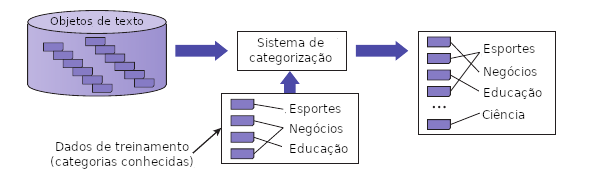
\includegraphics[width=0.75\textwidth]{img/figure15-1-zhai-traduzido.png}
    \end{center}
    \vspace{-0.0cm}
    \text{\footnotesize \textbf{Fonte:} Figura adaptada de \cite[p.~300]{Zhai2016TDMA}.}
    \label{fig:categorização-de-texto-zhai2016}
\end{figure}
    \end{frame}

    \begin{frame}{\sectiontitle{sec:introdução}}{Tarefa de classificação de texto}
        Processo de classificação de texto:
        \begin{itemize}
            \item Derivação de atributos;
            \item Manejo de atributos (\textit{feature engineering});
            \item Diferentes conjuntos de atributo impactam no desempenho dos classificadores de MT;
            \item Criação de atributos pode melhorar a acurácia.
        \end{itemize}
        \begin{block}{Recuperação de Informação na Classificação}
            \begin{itemize}
                \item Técnicas de RI são utilizadas intensivamente no pré-processamento dos textos para as tarefas de MT;
                \item Utilização de funções de ranqueamento de RI diretamente na criação de atributos é rara, somente foi encontrada as pesquisas de \cite{WEREN_MESTRADO_2014}.
            \end{itemize}
        \end{block}
    \end{frame}

    \begin{frame}{\sectiontitle{sec:introdução}}{Recuperação de Informação}
        Segundo \cite[p.~5--8]{Baeza-Yates2011}, a área de Recuperação de Informação abarca os seguintes processos aplicados sobre coleções de documentos:
        \begin{itemize}
            \item Armazenamento;
            \item Indexação;
            \item Recuperação; e
            \item Ranqueamento de consultas.
        \end{itemize}

        \begin{block}{Foco dos sistemas de RI}
            Segundo \cite[p.~2, tradução nossa]{KowalskiIRAA201}:
            \begin{itemize}
                \item O objetivo principal de um sistema de Recuperação de Informação é minimizar a sobrecarga do usuário em localizar informação de valor.
                Na perspectiva do usuário, sobrecarga pode ser definido como o tempo que decorre para localizar a informação necessária.
                O tempo inicia quando um usuário começa a interagir com o sistema e termina quando encontra os itens de interesse.
            \end{itemize}
        \end{block}
    \end{frame}

    \begin{frame}{\sectiontitle{sec:introdução}}{Recuperação de Informação}
        Recuperação de Informação:
        \begin{itemize}
            \item Área de estudo madura e bem desenvolvida;
            \item Complexa.
        \end{itemize}

        \begin{block}{Benefícios da utilização de ferramentas de RI já existentes}
            \begin{itemize}
                \item Implementar sistemas de RI que atendam os objetivos da área se torna dificultoso pela necessidade de otimização desses sistemas para atingir o estado da arte.

                \item É vantajoso usar ferramentas que subsidiem as tarefas de armazenamento, indexação, recuperação e ranqueamento da Recuperação de Informação.

                \item Facilidade no cálculo das funções de ranqueamento para criação de atributos derivados de RI em tarefas de MT.
            \end{itemize}
        \end{block}
    \end{frame}

    \begin{frame}{\sectiontitle{sec:introdução}}{Objetivo geral}

        \begin{block}{Objetivo geral}
            Avaliar o desempenho de atributos oriundos de Recuperação de Informação para tarefas de Mineração de Textos.
        \end{block}
    \end{frame}

    \begin{frame}{\sectiontitle{sec:introdução}}{Objetivos específicos}
        \begin{block}{Objetivos específicos}
            \begin{itemize}
        	\item Avaliar o ganho de desempenho de classificadores de Mineração de Texto com adição de atributos derivados da função de ranqueamento BM25 da Recuperação de Informação, em pelo menos 2 corpus de competições diferentes, utilizando medidas consolidadas na literatura;

        	\item Reproduzir soluções disponíveis \textit{online} para os corpus selecionados, comprovando as medidas dos resultados das competições;

            \item Elencar em qual dos corpus selecionados os atributos criados proporcionam maior ganho de desempenho de classificador;

            \item Comparar o desempenho computacional de ferramentas de armazenamento e indexação de textos:
            \begin{itemize}
                \item na questão de indexação;
                \item na questão de consulta utilizando as implementações do BM25 nativas das ferramentas;
            \end{itemize}

            % \item Avaliar, empiricamente, a facilidade de instalação, utilização e integração das ferramentas de armazenamento e indexação selecionadas.
            \end{itemize}
        \end{block}
    \end{frame}


\section{Fundamentação Teórica}\label{sec:fundamentação-teórica}

    % \begin{frame}{\sectiontitle{sec:fundamentação-teórica}}{Subtítulo da seção ou do slide}
    %     \begin{block}<+->{Exemplo de lista de itens}
    %     \begin{itemize}
    %     \item Item a.
    %     \item Item b.
    %     \item Item c.
    %     \end{itemize}
    %     \end{block}
    %     \begin{block}<+->{Exemplo de lista de itens numerada}
    %     \begin{enumerate}[<+-|alert@+>]
    %     \item Item numerado 1.
    %     \item Item numerado 2.
    %     \item Item numerado 3.
    %     \end{enumerate}
    %     \end{block}
    % \end{frame}

    \subsection{Recuperação de Informação}\label{subsec:RI}


    \begin{frame}{\sectiontitle{subsec:RI}}{A área de estudo}
        Desde o princípio dos registros físicos, os humanos tem uma certa preocupação com o armazenamento de informação e modos de obter informação, que é uma necessidade humana.

        \begin{block}{Evolução da transferência de informação}
            \begin{itemize}
                \item Consulta a outras pessoas;
                \item Registros físicos em papeis e similares;
                \item Meios digitais.
            \end{itemize}
        \end{block}

        % Devido ao volume enorme de conhecimento gerado pela humanidade é necessário otimizar a busca de informações específicas:
        % \item Sistemas de classificação de áreas e subáreas do conhecimento
        \begin{itemize}
            \item Otimização da busca de informações específicas:
            \begin{itemize}
                \item Sistemas manuais de classificação de áreas e subáreas do conhecimento;
            \end{itemize}
            \item Ineficácia dos sistemas manuais:
            \begin{itemize}
                \item Sistemas mecânicos no início do século 20;
                \item Sistemas computacionais na década de 1940.
            \end{itemize}
        \end{itemize}
        % Ainda assim sistemas manuais se tornaram ineficazes, surgiram, no início do século 20, os primeiros sistemas mecânicas de recuperação de informação.

        % Sistemas computacionais introduzidos na década de 1940 utilizados para consulta rápida de informações armazenadas.

        Necessidade de estabelecer algoritmos que retornem informação relevante aos usuários dos sistemas de RI.
    \end{frame}

    \begin{frame}{\sectiontitle{subsec:RI}}{A área de estudo}
        \begin{block}{Campo científico de Recuperação de Informação}
            Segundo \cite[p.~1]{Manning2008IIR}, Recuperação de Informação (RI, do inglês \textit{Information Retrieval}) consiste de encontrar material (geralmente documentos) de natureza desestruturada (geralmente texto) que satisfaça uma necessidade de informação dentro de grandes acervos (geralmente armazenados em computadores).
            \par
            Preocupações iniciais da área, segundo \cite[p.~3]{Sanderson2012THIRR}:
            \begin{enumerate}%[label=(\alph*)]
                \item \textit{como indexar documentos}; e
                \item \textit{como recuperá-los}.
            \end{enumerate}
        \end{block}
        \begin{itemize}
            \item Início baseado nos sistemas de indexação manuais;
            \item Migração para sistema baseado em palavras, Uniterm;
            \item Prevalência da indexação por palavras.
        \end{itemize}
        % Baseou-se nos sistemas de indexação manuais já consolidados no campo bibliotecário, como o CDD.

        % No entanto foi demonstrado que um sistema baseado em palavras, como o sistema Uniterm, era melhor.
        % A indexação por palavras prevaleceu.

    \end{frame}

    \begin{frame}[fragile = singleslide]{\sectiontitle{subsec:RI}}{Funcionamento de sistema de RI moderno}%
        % \begin{columns}[t]%
            % \column{0.475\textwidth}%
            \vspace{-0.5cm}
\begin{figure}[h]
    \centering
    \caption{Processos de indexação, recuperação, e ranqueamento dos documentos.}
    \begin{center}
        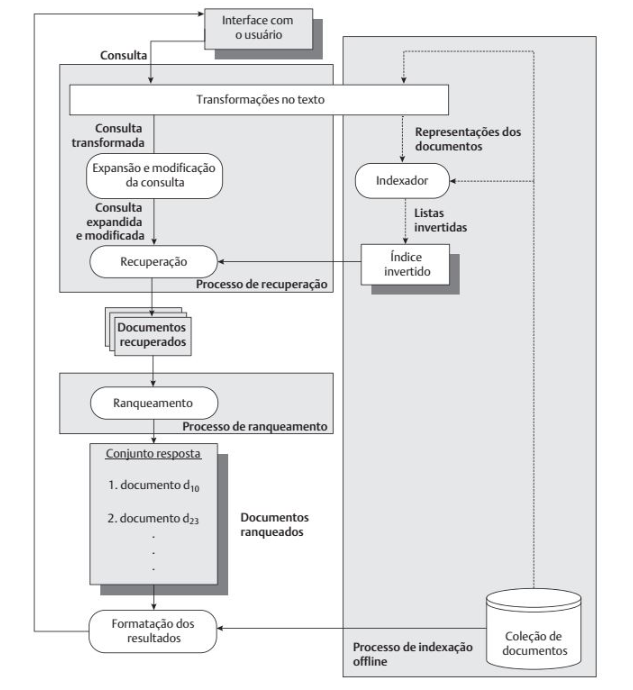
\includegraphics[width=0.37\textwidth]{img/baeza2013-figura-1-3.png}    
    \end{center}
    \vspace{-0.0cm}
    \text{\footnotesize \textbf{Fonte:} Figura extraída de \cite[p.~8]{Baeza-Yates2011}.}
    \label{fig:diagrama-baeza2013-fig1-3}
\end{figure}%
        % \end{columns}
    \end{frame}

    \begin{frame}[fragile = singleslide]{\sectiontitle{subsec:RI}}{Vocabulário}
        \begin{itemize}
            \item Termo: sinônimo de palavra;
            \item Documento: objeto digital que contém dados textuais, contém termos;
            \item Coleção de documentos: o conjunto de documentos disponíveis num sistema de RI;
            \item Consulta: sequência de termos que representam uma necessidade de informação.
        \end{itemize}
    \end{frame}

    \begin{frame}[fragile = singleslide]{\sectiontitle{subsec:RI}}{Métodos booleanos}
        \begin{table}[H]
    \centering
    \caption{Matriz de incidência de termo-documento do livro \textit{Shakespeare’s Collected Works}. Cada elemento (i, j) da matriz é 1 se a peça de teatro na coluna j contém a palavra na linha i, caso contrário o elemento é 0.}
    \begin{adjustbox}{max width=0.8\textwidth}
        \begin{tabular}{|c|c|c|c|c|c|c|c}
            \hline
            \diagbox{Palavra}{
                \raisebox{-1.27cm}{
                    \rotatebox{90}{
                        \parbox{1.6cm}{\centering Peça \\ de teatro}
                    }
                }
            } 
            & \makecell{Antony \\ and \\ Cleopatra} 
            & \makecell{Julius \\ Caesar} 
            & The Tempest 
            & Hamlet 
            & Othello 
            & Macbeth 
            & ... 
            \\ \hline
            Antony     & 1 & 1 & 0 & 0 & 0 & 1 & \\
            Brutus     & 1 & 1 & 0 & 1 & 0 & 0 & \\
            Caeasar    & 1 & 1 & 0 & 1 & 1 & 1 & \\
            Calpurnia  & 0 & 1 & 0 & 0 & 0 & 0 & \\
            Cleopatra  & 1 & 0 & 0 & 0 & 0 & 0 & \\
            mercy      & 1 & 0 & 1 & 1 & 1 & 1 & \\
            worser     & 1 & 0 & 1 & 1 & 1 & 0 & \\
            ...        & & & & & & & 
        \end{tabular}
    \end{adjustbox}
    \text{\footnotesize \textbf{Fonte:} Tabela adaptada de \cite[p.~4]{Manning2008IIR}.}
    \label{tab:matriz-incidência-termo-documento}
\end{table}
    \end{frame}

    \begin{frame}[fragile = singleslide]{\sectiontitle{subsec:RI}}{Ranqueamento}
        Recuperação ranqueada:
        \begin{itemize}
            \item Estabelece uma pontuação para cada resultado;
            \item Retorno dos resultados de forma ordenada.
        \end{itemize}

        Contabilização do número de aparições de cada um dos termos no documento.
        \begin{itemize}
            \item Número de ocorrências do termo \textit{t} em um documento \textit{d}:
            \begin{equation}\label{eq:tf-td}
                \text{tf}_{\text{\textit{t},\textit{d}}}
            \end{equation}
            \item Relevância dos termos na coleção de documentos:
            \begin{equation}
                \label{eq:inverse-document-frequency}
                \text{idf}_{\text{\textit{t}}} = \log{\frac{N}{\text{df}_{\text{\textit{t}}}}}
            \end{equation}

            \begin{equation}
                \label{eq:tf-idf}
                \text{tf-idf}_{\text{\textit{t},\textit{d}}}  = \text{tf}_{\text{\textit{t},\textit{d}}} \times \text{idf}_{\text{\textit{t}}}.
            \end{equation}
        \end{itemize}

    \end{frame}

    \begin{frame}[fragile = singleslide]{\sectiontitle{subsec:RI}}{Recuperação ranqueada: exemplo de tf--idf}
        \begin{columns}[t]
            \column{0.67\textwidth}
            \begin{table}[h]
    \centering
    \caption{Exemplo de cálculo do valor de tf-idf.}
    \begin{adjustbox}{max width=1.0\textwidth}
        \begin{tabular}{|l|r|r|r|r|r|r|r|r|}
            \hline
            \multicolumn{3}{|l|}{
                \diagbox[width=4.75cm, height=2.55cm]{Termo}{
                    \raisebox{-1.87cm}{
                        \rotatebox{90}{
                            \parbox{1.6cm}{\centering Documento}
                        }
                    }
                }
            } 
            & \multicolumn{2}{|c|}{D\textsubscript{1}} 
            & \multicolumn{2}{|c|}{D\textsubscript{2}} 
            & \multicolumn{2}{|c|}{D\textsubscript{3}} 
            \\ \hline
            & $\text{df}_{\text{\textit{t}}}$ & $\text{idf}_{\text{\textit{t}}}$ & $\text{tf}_{\text{\textit{t},\textit{d}}}$ & $\text{tf-idf}_{\text{\textit{t},\textit{d}}}$ & $\text{tf}_{\text{\textit{t},\textit{d}}}$ & $\text{tf-idf}_{\text{\textit{t},\textit{d}}}$ & $\text{tf}_{\text{\textit{t},\textit{d}}}$ & $\text{tf-idf}_{\text{\textit{t},\textit{d}}}$ \\ \hline
            car        & 18165 & 1,65 & 27 & 44,55 & 4 & 6,6 & 24 & 39,6 \\
            auto       & 6723  & 2,08 & 3  & 6,24 & 33 & 68,64 & 0 & 0 \\
            insurance  & 19241 & 1,62 & 0  & 0 & 33 & 54,46 & 29 & 46,98 \\
            best       & 25235 & 1,5  & 14 & 21 & 0 & 0 & 17 & 25,5
        \end{tabular}
    \end{adjustbox}
    \text{\footnotesize \textbf{Fonte:} Tabelas disponíveis em \cite[p.~109--110]{Manning2008IIR}.}
    \label{tab:exemplo-tf-idf}
\end{table}

            \column{0.30\textwidth}
            \begin{equation}
                \label{eq:pontuação-simples-tf-idf}
                \text{Pontuação(\textit{q},\textit{d})} = \sum_{\textit{t} \in \textit{q}}^{} \text{tf-idf}_{\text{\textit{t},\textit{d}}}.
            \end{equation}

            \vspace{1cm}

            $\text{Pontuação(\{\textit{auto},\textit{car}\},D\textsubscript{x})}$ para cada documento:
            \begin{itemize}
                \setlength\itemsep{-0.2em}
                \item D\textsubscript{1}: 50,79
                \item D\textsubscript{2}: 75,24
                \item D\textsubscript{3}: 39,60
            \end{itemize}
        \end{columns}
    \end{frame}

    \begin{frame}[fragile = singleslide]{\sectiontitle{subsec:RI}}{Recuperação ranqueada: Modelo de espaço vetorial}
        Modelo de espaço vetorial:
        \begin{itemize}
            \item Surge a partir das limitações do modelo booleano;

            \item Representação dos documentos em um espaço vetorial comum.
        \end{itemize}


        \begin{block}{Vantagens do modelo vetorial}
            \begin{itemize}
                \item Melhora da qualidade dos resultados;

                \item Capacidade de correspondência parcial;

                \item Organização dos resultados pelo grau de similaridade com a consulta; e

                \item Normalização dos tamanhos dos documentos.
            \end{itemize}
        \end{block}
    \end{frame}

    \begin{frame}[fragile = singleslide]{\sectiontitle{subsec:RI}}{Recuperação ranqueada: Modelo de espaço vetorial}
        Representação dos documentos e das consultas:
        \begin{itemize}
            \item Vetores $t$-dimensionais;
            \item Pesos de cada termo são associados.
        \end{itemize}
        \begin{equation}
            \label{eq:vetor-pesos-documento}
    		\vec{d_j} = (w_{1,j}, w_{2,j}, \cdots , w_{t,j})
        \end{equation}
        \begin{equation}
            \label{eq:vetor-pesos-consulta}
    		\vec{q} = (w_{1,q}, w_{2,q}, \cdots , w_{t,q})
        \end{equation}

        \begin{block}{Padrão de peso mais utilizado}
            \begin{equation}
                \text{tf-idf}_{\text{\textit{t},\textit{d}}}
            \end{equation}

            Segundo \cite[p.~77--78]{Baeza-Yates2011}, como $w_{i,q}$ é o peso associado com o par termo-consulta $(k_i, q)$, a aplicação do $\text{tf-idf}_{\text{\textit{t},\textit{d}}}$ vira $\text{tf-idf}_{k_i\text{,}\textit{q}}$ para os pesos associados à uma consulta $q$.
        \end{block}
    \end{frame}


    \begin{frame}[fragile = singleslide]{\sectiontitle{subsec:RI}}{Recuperação ranqueada: exemplo do modelo vetorial}
        \begin{columns}[t]
            \column{0.50\textwidth}
            \begin{figure}[H]
    \centering
    \caption{O cosseno de $\theta$ é adotado como $\text{Pontuação}(\vec{d_j},\vec{q})$. }
    \begin{center}
        \begin{tikzpicture}[scale=1.25]
            \coordinate[label=below  left:""] (A) at (-1.5cm,-1.cm);
            \draw[-Stealth]
                (A) to ["",sloped] ++ ({atan(2/3)}:{sqrt(4+9)})  coordinate[label=above right:$d_j$] (B);
            \draw[-Stealth] 
                (A) to ["" ']      ++ (0:3)                      coordinate[label=below right:q] (C);
            \pic ["$\theta$", draw, angle radius = 12mm, angle eccentricity=1.3]     
                {angle = C--A--B};
        \end{tikzpicture}
    \end{center}
    \vspace{-0.0cm}
    \text{\footnotesize \textbf{Fonte:} Baseado na figura disponível em \cite[p.~78]{Baeza-Yates2011}.}
    \label{fig:similaridade-cosseno}
\end{figure}

% \begin{figure}[H]
%     \centering
%     \includegraphics[width=1.0\textwidth]{img/estrategico.png}
%     \caption{Planejamento estratégico da BSS Tecnologias.}
%     \label{fig:similaridade-cosseno}
% \end{figure}

            \column{0.45\textwidth}
            \vspace{1cm}
            \begin{block}{Função de ranqueamento}
            \begin{equation}
                \label{eq:pontuação-similaridade-cosseno}
        		\text{Pontuação\_COS}(\vec{d_j}, \vec{q}) = \frac{\vec{d_j} \bullet \vec{q} }{ \norm{\vec{d_j}} \times \norm{\vec{q}} }
            \end{equation}
            \end{block}
            \vspace{1cm}

        \end{columns}
    \end{frame}

    \begin{frame}[fragile = singleslide]{\sectiontitle{subsec:RI}}{Recuperação ranqueada: modelo probabilístico}
        Modelos probabilísticos:
        \begin{itemize}
            \item Partem do princípio da incerteza da relevância dos documentos retornados (PRP);
            \item Função de ranqueamento definida estatisticamente como $P(R = 1| d,q)$ onde $R \in \{0, 1\}$ é uma variável binária aleatória que denota a relevância.
        \end{itemize}

        Segundo \cite[p.~333]{robertson_probabilistic_2010}, o
        princípio do ranqueamento probabilístico (PRP) é a base para o chamado \textit{Framework} de Relevância Probabilística o qual, por sua vez, deu origem aos:
        \begin{itemize}
            \item Modelo de independência binária (BIM);
            \item Modelos de \textit{feedback} de relevância;
            \item BM25; e a
            \item Diversas variações do BM25.
        \end{itemize}
    \end{frame}

    \begin{frame}[fragile = singleslide]{\sectiontitle{subsec:RI}}{Recuperação ranqueada: modelo probabilístico - Okapi BM25}
        Função de ranqueamento Okapi BM25:
        \begin{itemize}
            \item Evolução das implementações do BIM;
            \item Integra conceitos aplicados no modelo vetorial:
                \begin{itemize}
                    \item Frequência dos termos;
                    \item Normalização de tamanho; e
                    \item Correspondência parcial.
                \end{itemize}
            \item Alguns autores, como \cite[p.~111]{Zhai2016TDMA}, apresentam a função BM25 junto às dos modelos vetoriais devido à sua similaridade com estes.
        \end{itemize}

        \begin{block}{Função de ranqueamento BM25}
            \begin{equation}
                \label{eq:okapi-bm25}
        		\text{Pontuação\_BM25}(d_j, q) = \sum_{t \in q} \text{idf}_{\text{\textit{t}}}
        		\cdot
        		\frac{(k_1 + 1) \text{tf}_{t,d}}{k_1((1-b)+b \times (\frac{L_d}{L_{\text{avg}}})) + \text{tf}_{t,d}}
            \end{equation}
        \end{block}
        Os termos $\text{tf}_{t,d}$ e $\text{idf}_{\text{\textit{t}}}$ tem o mesmo significado já apresentado nos modelos anteriores.
        Os termos $b$ e $k_1$ são parâmetros de refinamento.
    \end{frame}

    \begin{frame}[fragile = singleslide]{\sectiontitle{subsec:RI}}{Recuperação ranqueada: modelo probabilístico - Okapi BM25}
        \begin{block}{Função de ranqueamento BM25}
            \begin{equation}
                \label{eq:okapi-bm25}
        		\text{Pontuação\_BM25}(d_j, q) = \sum_{t \in q} \text{idf}_{\text{\textit{t}}}
        		\cdot
        		\frac{(k_1 + 1) \text{tf}_{t,d}}{k_1((1-b)+b \times (\frac{L_d}{L_{\text{avg}}})) + \text{tf}_{t,d}}
            \end{equation}
        \end{block}
        \begin{itemize}
            \item $\text{tf}_{t,d}$: contagem do número de ocorrências do termo $t$ no documento $d$;

            \item $\text{idf}_{\text{\textit{t}}}$: peso de Robertson/Spark Jones dado pela seguinte fórmula:
            \begin{equation}
                \label{eq:peso-rsj-adaptado}
        		\text{idf}_{\text{\textit{t}}} = \log{\frac{N-\text{df}_{\text{\textit{t}}}+\frac{1}{2}}{\text{df}_{\text{\textit{t}}} + \frac{1}{2} }}.
            \end{equation}
            Mas pode ser simplificado para o valor já apresentado nos modelos anteriores;

            \item $L_{\text{avg}}$: tamanho médio dos documentos na coleção inteira;

            \item $L_d$: tamanho do documento;

            \item $b$ ($0 \leq b \leq 1$): controle do grau de normalização por tamanho de documento. Usa como referência os valores de $L_{\text{avg}}$ e $L_d$;

            \item $k_1$ ($0 \leq k_1 \leq \infty$): efeito da correção de frequência dos termos presente na fórmula.
        \end{itemize}
    \end{frame}

    \begin{frame}[fragile = singleslide]{\sectiontitle{subsec:RI}}{Recuperação ranqueada: modelo probabilístico - Okapi BM25}
        Consultas com muitos termos, e repetição destes, podem ser consideradas também pela função Okapi BM25 com a adição de um fator de ajuste $k_3$.

        \begin{block}{Função de ranqueamento BM25 adaptada para termos da consulta}
            \begin{equation}
                \label{eq:okapi-bm25-tf-consulta}
        		\text{Pontuação\_BM25}(d_j, q) =
        		\sum_{t \in q}
        		\Bigg[ \log{\frac{N}{\text{df}_{t}}} \Bigg]
        		\cdot
        		\frac{(k_1 + 1) \text{tf}_{t,d}}{k_1((1-b)+b \times (\frac{L_d}{L_{\text{avg}}})) + \text{tf}_{t,d}} \cdot
        		\frac{(k_3+1) \text{tf}_{t,q}}{k_3 + \text{tf}_{t,q}}
            \end{equation}
        \end{block}
        \begin{itemize}
            \item Parâmetros de refinamento $b$, $k_1$ e $k_3$ são definidos para otimizar o desempenho na recuperação em uma coleção de teste.
            \item Valores experimentais:
                \begin{itemize}
                    \item $k_1$ e $k_3$: valores entre $1.2$ e $2$;
                    \item $b = 0.75$ ou valores entre $0.5$ e $0.8$.
                \end{itemize}
        \end{itemize}
    \end{frame}

    \subsection{Mineração de Texto}\label{subsec:MT}

    \begin{frame}[fragile = singleslide]{\sectiontitle{subsec:MT}}{Extração do conhecimento de dados textuais}
        \begin{columns}[t]
        \column{0.45\textwidth}

        A Mineração de Textos (MT) é definida como o processo de extrair conhecimento implícito de dados textuais \cite{Jo2018TMCIBDC,Feldman:2006:TMH:1076381}.

        \begin{itemize}
            \item Tratada como \textit{knowledge discovery in text} por alguns autores, \cite{Kodratoff:1999:KDT:646358.689959} e \cite{Feldman:1995:KDT:3001335.3001354}.

            \item Recebe suporte direto da Mineração de Dados.

            \item Mineração de Dados é somente uma parte do processo de descoberta de conhecimento \cite[p.~6]{Han:2011:DMC:1972541}.
        \end{itemize}

        \column{0.45\textwidth}
        \begin{block}{Processo de descoberta de conhecimento em dados}
            Composto pelas seguintes etapas, segundo \cite[p.~6--7]{Han:2011:DMC:1972541}:
            \begin{enumerate}
                \item \textbf{Limpeza dos dados}; %: remoção de ruído e dados inconsistentes;

                \item \textbf{Integração dos dados}; %: combinação de múltiplas fontes de dados;

                \item \textbf{Seleção dos dados}; %: dados relevantes para a tarefa de análise são recuperados do banco de dados;

                \item \textbf{Transformação dos dados}; %: dados são transformados e consolidados em formas apropriadas para mineração sendo realizadas, por exemplo, ações de agregação ou resumo;

                \item \textbf{Mineração dos dados}; %: métodos inteligentes são aplicados para extrair padrões de dados;

                \item \textbf{Avaliação de padrões}; e %: são identificados os padrões que realmente tão interessantes para representar o conhecimento baseado em medidas de nível de interesse;
                \item \textbf{Apresentação do conhecimento}. %: o conhecimento minerado é apresando aos usuários por meio de técnicas de visualização e representação de conhecimento.
            \end{enumerate}
        \end{block}
        \end{columns}
    \end{frame}

    \begin{frame}[fragile = singleslide]{\sectiontitle{subsec:MT}}{O processo de descoberto do conhecimento (KDD)}
        \vspace{-0.5cm}
\begin{figure}[h]
    \centering
    \caption{Mineração de dados como uma fase do processo de descoberta do conhecimento (KDD).}
    \begin{center}
        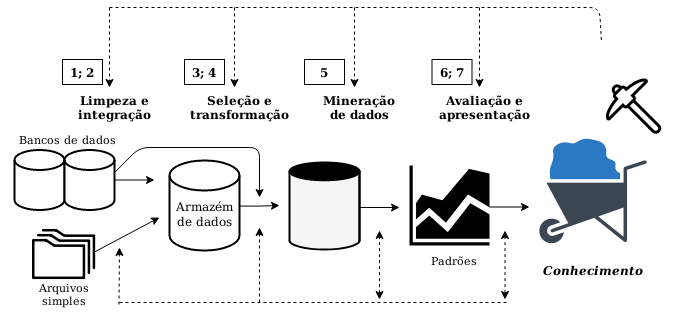
\includegraphics[width=0.85\textwidth]{img/based-on-figure-1-4-han-2011.png}
    \end{center}
    \vspace{-0.0cm}
    \caption{\footnotesize \textbf{Fonte:} Figura baseada na original de \cite[p.~7]{Han:2011:DMC:1972541}.}
    \label{fig:diagrama-mineração-texto-han}
\end{figure}
    \end{frame}

    \begin{frame}[fragile = singleslide]{\sectiontitle{subsec:MT}}{Pré-processamento}
        \begin{itemize}
            \item Mineração de Dados assume que os dados já estão processados.
            \begin{itemize}
                \item Pré-processamento do KDD direcionado à limpeza e integração dos dados, etapas 1 e 2.
            \end{itemize}

            \item Mineração de Texto trabalho com dados desestruturados.
                \begin{itemize}
                    \item Pré-processamento focado em mais extração de atributos, etapas 3 e 4.
                \end{itemize}

            \item O pré-processamento da MT utiliza de técnicas da:
            \begin{itemize}
                \item Recuperação de Informação;
                \item Extração de informação; e
                \item Linguística computacional.
            \end{itemize}
            para transformar as coleções de documentos desestruturados em dados intermediários cuidadosamente estruturados \cite[p.~2--3]{Feldman:2006:TMH:1076381}.

            \item Estrutura intermediária definida por um modelo representacional dos documentos de texto composto por um conjunto de atributos.
        \end{itemize}
    \end{frame}

    \begin{frame}[fragile = singleslide]{\sectiontitle{subsec:MT}}{Diferença entre MT e RI}
        Apesar da Mineração de Texto utilizar de técnicas da Recuperação de Informação, ambos são campos independentes com objetivos diferentes.

        \begin{block}{Diferença entre MT e RI}
            \cite[p.~4, tradução nossa]{Jo2018TMCIBDC} ressalta as diferenças:
            \begin{itemize}
                \item A saída da mineração de dados é o conhecimento implícito que é necessário diretamente para a tomada de decisões, enquanto a saída da recuperação é composta por alguns dos itens de dados que são relevantes para a consulta dada.
                Por exemplo, no domínio de preços de ações, a previsão dos preços futuros de ações é uma tarefa típica da mineração de dados, enquanto que obter alguns dos preços de ações passadas e atuais é tarefa da recuperação de informação.
                Observe que a certeza perfeita nunca existe na mineração de dados, em comparação com a recuperação.
                A computação mais avançada para obter conhecimento dos dados brutos, chamada de síntese, é necessária para executar as tarefas de mineração de dados.
            \end{itemize}
        \end{block}
    \end{frame}

    \begin{frame}{\sectiontitle{subsec:MT}}{Diferença entre MT e RI}
        \begin{table}[H]
    \centering
    \caption{Mineração de Dados versus Recuperação de Informação (em específico para objetos de texto a comparação vale para Mineração de Texto versus Recuperação de Texto).}
    \begin{adjustbox}{max width=0.8\textwidth}
    \begin{tabular}{|l|l|l|}
        \hline
         
        & \makecell[l]{\textbf{Mineração}}
        & \makecell[l]{\textbf{Recuperação}}
        \\ \hline
        Saída
        & Conhecimento 
        & Itens relevantes
        \\ \hline
        Exemplo
        & Valores previstos 
        & Valores anteriores ou atuais
        \\ \hline
        Certeza
        & Probabilística 
        & Nítida
        \\ \hline
        Síntese
        & Necessária 
        & Opcional
        \\ 
        \hline
    \end{tabular}
    \end{adjustbox}
    
    \text{\footnotesize \textbf{Fonte:} \cite[p.~4]{Jo2018TMCIBDC}.}
    \label{tab:mineração-vs-recuperação}
\end{table}
    \end{frame}

    \begin{frame}{\sectiontitle{subsec:MT}}{Corpus}
        \begin{itemize}
            \item Vários formatos de texto são utilizados para o processamento computacional de texto:
            \begin{itemize}
                \item MS Word com extensão ``doc'';
                \item MS PowerPoint com extensão ``ppt'';
                \item MS Excel com o ``xls'';
                \item PDF para transferência entre computadores.
            \end{itemize}
            \item Texto simples, ou texto sem formatação, é o formato mais elementar de texto que é feito por um editor de texto.

            \item Corpus é uma coleção de textos simples, referenciada pelo diretório que contém os arquivos de texto \cite[p.~6]{Jo2018TMCIBDC}.

            \item \cite[p.~9]{KwartlerTMPWR2017} considera como corpus qualquer corpo, ou conjunto, grande de texto organizado.
        \end{itemize}
    \end{frame}

    \begin{frame}{\sectiontitle{subsec:MT}}{Corpus: exemplo de arquivo de texto simples}
        \begin{figure}[h]
    \centering
    \caption{Arquivo de texto simples, texto não formatado, aberto para edição no xed.}
    \begin{center}
        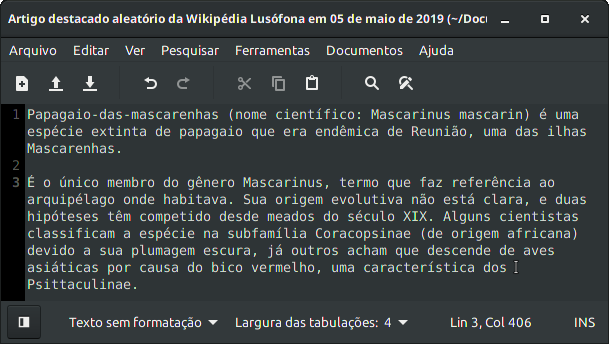
\includegraphics[width=0.60\textwidth]{img/exemplo-texto-simples.png}
    \end{center}
    \vspace{-0.0cm}
    \text{\footnotesize \textbf{Fonte:} O autor, conteúdo do texto obtido de \cite{Wikipedia_ConteudoDest05maio_2019}.}
    \label{fig:exemplo-texto-simples}
\end{figure}


    \end{frame}

    \begin{frame}[fragile = singleslide]{\sectiontitle{subsec:MT}}{Corpus: exemplo de arquivo XML}
        \begin{figure}[h]
    \centering
    \caption{Exemplo de documento XML aberto no editor xed.}
    \begin{center}
        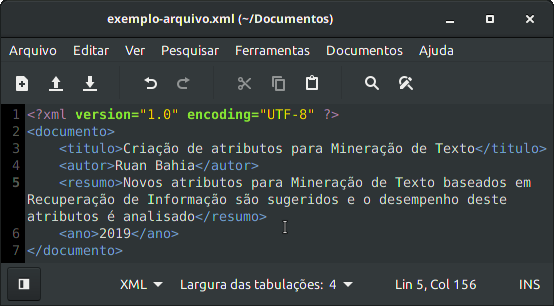
\includegraphics[width=0.60\textwidth]{img/exemplo-arquivo-xml.png}
    \end{center}
    \vspace{-0.0cm}
    \text{\footnotesize \textbf{Fonte:} O autor.}
    \label{fig:exemplo-arquivo-xml}
\end{figure}
    \end{frame}


    \begin{frame}[fragile = singleslide]{\sectiontitle{subsec:MT}}{Tarefas da Mineração de Dados}
        \begin{columns}[t]
        \column{0.30\textwidth}
        Segundo \cite[p.~7]{TanIDM2014} e \cite[p.~15]{Han:2011:DMC:1972541} são separadas em:
        \begin{itemize}
            \item Descritivas; e
            \item Preditivas.
        \end{itemize}

        As tarefas descritivas são de:
        \begin{itemize}
            \item Agrupamento;
            \item Associação;
            \item Descrição; e
            \item Detecção de anomaliaas.
        \end{itemize}

        \column{0.65\textwidth}
        \vspace{-1.0cm}
\begin{figure}[h]
    \centering
    \caption{As quatro principais tarefas da mineração de dados.}
    \begin{center}
        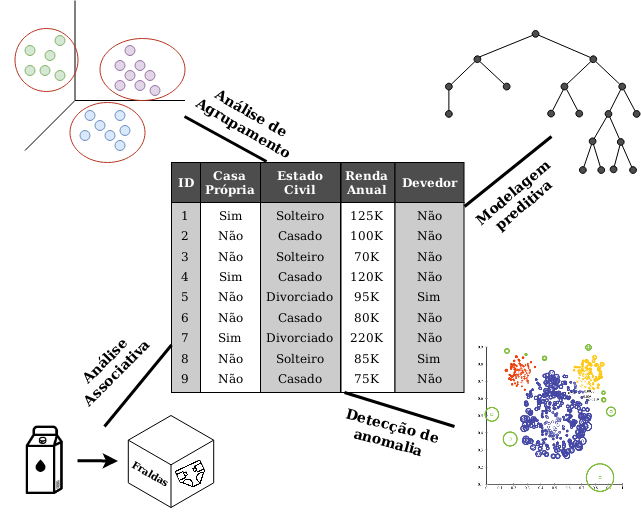
\includegraphics[width=0.75\textwidth]{img/tarefas-principais-mineracao-dados.png}
    \end{center}
    \vspace{-0.0cm}
    \text{\footnotesize \textbf{Fonte:} Figura baseada na original de \cite[p.~7]{TanIDM2014}.}
    \label{fig:tarefas-principais-mineração-dados}
\end{figure}


        \end{columns}
    \end{frame}

    \begin{frame}[fragile = singleslide]{\sectiontitle{subsec:MT}}{Tarefas da Mineração de Dados: Classificação binária}
        \begin{itemize}
            \item O problema da classificação consiste na aprendizagem da estrutura dos exemplos do conjunto de dados, os quais estão classificados em grupos chamados de categorias ou classes \cite[p.~285]{Aggarwal_DMTT_2015}.

            \item \cite[p.~146, tradução nossa]{TanIDM2014} dizem que ``classificação é a tarefa de aprender uma função objetivo $f$ que mapeia cada conjunto de atributos $x$ a um rótulo de classe predefinido $y$''.

            \item Segundo \cite[p.~286]{Aggarwal_DMTT_2015}, a maior parte dos algoritmos de classificação possui duas fases:
            \begin{enumerate}
                \item \textbf{Fase de treinamento};
                \item \textbf{Fase de teste};
            \end{enumerate}

            \item A classificação binária é o caso mais simples das tarefas de classificação, pois nele só existem duas possibilidades de rótulo de classe e cada objeto de dados pertence, exclusivamente, a uma das classes.
        \end{itemize}
    \end{frame}

    \begin{frame}[fragile = singleslide]{\sectiontitle{subsec:MT}}{Engenharia de Atributos}
        \begin{itemize}
            \item \cite{ZhengFEML2018} chamam de \textit{manejo de atributos} o processo para extrair atributos passíveis de serem utilizados por classificadores da mineração de dados.

            \item \cite[p.~3, tradução nossa]{DongFEMLDA2018} definem \textit{feature engineering} como uma área que abrange ``os tópicos de transformação de atributos, geração de atributos, extração de atributos, seleção de atributos, análise e avaliação de atributos, metodologias de manejo generalista e automatizado de atributos, e aplicações do manejo de atributos''.

            Os tópicos da engenharia de atributos são:
            \begin{itemize}
                \item \textbf{Transformação de atributos};

                \item \textbf{Geração de atributos};

                \item \textbf{Seleção de atributos};

                \item \textbf{Metodologias de manejo generalista e automatizado de atributos};

                \item \textbf{Aplicações do manejo de atributos}.
            \end{itemize}
        \end{itemize}

    \end{frame}

    \begin{frame}[fragile = singleslide]{\sectiontitle{subsec:MT}}{Engenharia de Atributos: Atributos comuns para documentos}
        Os tipos de atributos mais utilizados para representar documentos, segundo  \cite[p.~5--7]{Feldman:2006:TMH:1076381}:
        \begin{itemize}
            \item \textbf{Caracteres}: são as letras, números, e caracteres especiais presentes nos documentos utilizados para construir a semântica do mesmo;

            \item \textbf{Palavras}: são símbolos linguísticos nativos do espaço de atributos de um documento.
            Atributos a nível de palavra geralmente são palavras únicas selecionadas de um documento nativo, e também é possível que sejam utilizados todas as palavras de um documento para representá-lo;

            \item \textbf{Termos}: são palavras únicas e frases com mais de uma palavra selecionadas de um corpus de documentos nativos por meio de técnicas específicas para extração de termos;

            \item \textbf{Conceitos}: são os atributos gerados de modo manual, baseado em regras, ou via categorização híbrida feita no pré-processamento.
            Por exemplo, um documento sobre carros esportivos pode não incluir a palavra ``automóvel'', mas este conceito pode ser utilizado para identificar e representar esse documento.
        \end{itemize}

    \end{frame}

    \begin{frame}[fragile = singleslide]{\sectiontitle{subsec:MT}}{Engenharia de Atributos: Criação de atributos}
        A criação de atributos consiste em derivar novos conjuntos de atributos que capturem, de forma mais efetiva, a informação carregada pelos dados \cite[p.~55]{TanIDM2014}.

        Metodologias de criação de atributos apresentadas por \cite[p.~55--57]{TanIDM2014}:
        \begin{itemize}
            \item \textbf{Extração de atributos}: a criação de um novo conjunto de atributos a partir dos dados brutos.

            \item \textbf{Mapeamento dos dados para um novo espaço}: mudar completamente a visualização dos dados.

            \item \textbf{Construção de atributos}: os atributos presentes nos dados possuem a informação necessária para o processo de mineração, mas não estão na forma adequada, assim novos atributos podem ser construídos na forma adequada.
        \end{itemize}

    \end{frame}

    \begin{frame}[fragile = singleslide]{\sectiontitle{subsec:MT}}{Medidas de avaliação de classificadores}
        \begin{columns}[t]
            \column{0.35\textwidth}
            \vspace{0.3cm}
            \begin{itemize}
                \item Verdadeiros positivos (\textit{TP});

                \item Verdadeiros negativos (\textit{TN});

                \item Falsos positivos (\textit{FP});

                \item Falsos negativos (\textit{FN}).
            \end{itemize}

            \column{0.62\textwidth}
            \begin{table}[H]
    \centering
    \caption{Matriz de confusão para uma tarefa de classificação binária, exibida com os totais para exemplos positivos e negativos.}
    \begin{adjustbox}{max width=0.8\textwidth}
    \begin{tabular}{l|p{1.2cm}|p{1.2cm}|p{1.2cm}|p{1.2cm}}
        \multicolumn{2}{c}{} 
        & \multicolumn{2}{c}{\textbf{Classe prevista}} 
        \\ \cline{3-4}
        \multicolumn{2}{c|}{}
        & \makecell[c]{\textit{sim}}
        & \makecell[c]{\textit{não}}
        & \makecell[c]{Total}
        \\ \cline{2-4}
        \multirow{2}{1.2cm}{
            \raisebox{0.0cm}{
                \rotatebox{90}{
                    \parbox{1.0cm}{\centering \textbf{Classe real}}
                }
            }
        }
        & \makecell[c]{\textit{sim}} 
        & \makecell[c]{\textit{TP}} 
        & \makecell[c]{\textit{FN}} 
        & \makecell[c]{$P$}
        \\ \cline{2-4}
        
        & \makecell[c]{\textit{não}} 
        & \makecell[c]{\textit{FP}}
        & \makecell[c]{\textit{TN}}
        & \makecell[c]{$N$}
        \\ \cline{2-4}
        \multicolumn{1}{c}{}
        & \multicolumn{1}{c}{Total} 
        & \multicolumn{1}{c}{$P`$}
        & \multicolumn{1}{c}{$N`$}
        & \multicolumn{1}{c}{$P + N$}
        \\
    \end{tabular}
    \end{adjustbox}
    \text{\footnotesize \textbf{Fonte:} Tabela disponível em \cite[p.~366]{Han:2011:DMC:1972541}.}
    \label{tab:matriz-confusão}
\end{table}
        \end{columns}
    \end{frame}

        \begin{frame}[fragile = singleslide]{\sectiontitle{subsec:MT}}{Medidas de avaliação de classificadores}
        \begin{columns}[t]
            \column{0.30\textwidth}
            \begin{itemize}
                \item Precisão ($p$);

                \item Revocação ($r$);

                \item $F$-\textit{score};

                \item Acurácia ($acc$);

                \item $F_\beta{}$.
            \end{itemize}

            \column{0.65\textwidth}

            \begin{equation}
                \label{eq:medida-precisão}
        		p =
        		\frac{\textit{TP}}{\textit{TP} + \textit{FP}}
        		= \frac{\textit{TP}}{P`}
            \end{equation}

            \begin{equation}
                \label{eq:medida-revocação}
        		r =
        		\frac{\textit{TP}}{\textit{TP} + \textit{FN}}
        		= \frac{\textit{TP}}{P}
            \end{equation}

            \begin{equation}
                \label{eq:medida-f-score}
        		F =
        		\frac{2 \times p \times r}{p + r}
            \end{equation}

            \begin{equation}
                \label{eq:medida-acurácia}
        		acc =
        		\frac{\textit{TP} + \textit{TN}}{P + N}
            \end{equation}

            \begin{equation}
                \label{eq:medida-f-beta}
        		F_\beta{} =
        		\frac{(1 + \beta{}^2) \times p \times r}{\beta{}^2 \times p + r}
            \end{equation}
        \end{columns}
    \end{frame}

\section{Material e Métodos}\label{sec:matmet}

    \begin{frame}{\sectiontitle{sec:matmet}}{Metodologia proposta}
        \begin{columns}[t]
            \column{0.30\textwidth}
            A metologia proposta para avaliação do desempenho dos atributos criados consiste dos seguinte passos:

            \begin{enumerate}
                \item \textbf{Corpus para Avaliação}
                \item \textbf{Armazenamento e Indexação em  SGBD NoSQL}
                \item \textbf{Transformação dos dados com adição dos atributos de RI}
                \begin{enumerate}
                    \item \textbf{Consultas}
                \end{enumerate}
                \item \textbf{Avaliação do Modelo}

                \item \textbf{Mineração dos Dados}
            \end{enumerate}

            \column{0.65\textwidth}
            \vspace{-0.9cm}
\begin{figure}[H]
    \centering
    \caption{Metodologia proposta para avaliação de desempenho, em verde estão as variáveis mensuráveis sugeridas.}
    \begin{center}
        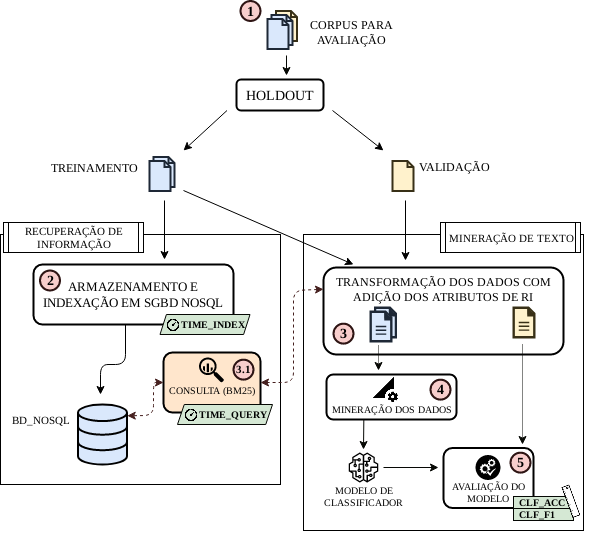
\includegraphics[width=0.72\textwidth]{img/diagrama-metodologia-v2-3.png}
    \end{center}
    \vspace{-0.0cm}
    \text{\footnotesize \textbf{Fonte:} O autor.}
    \label{fig:diagrama-da-metodologia}
\end{figure}
        \end{columns}
    \end{frame}

    \begin{frame}{\sectiontitle{sec:matmet}}{Corpus para avaliação}
        Definidos dois corpus de competições promovidas pela PAN\footnote{Sigla da organização que se originou do \textit{International Workshop on Plagiarism Analysis, Authorship Identification, and Near-Duplicate Detection} em 2007 \cite{PAN_Workshop_2007}.}:
        \begin{itemize}
            \item \textbf{DB\_AUTHORPROF - \textit{Author Profiling - PAN @ CLEF 2018}:} Uma tarefa da competição \textit{CLEF 2018} promovida pela PAN na classe de análise de autoria, a qual foca na identificação de gênero no Twitter em três linguagens distintas, inglês, espanhol, e árabe \cite{PAN_APCLEF_2018}.

            \item \textbf{DB\_HYPARTISAN - \textit{Hyperpartisan News Detection - PAN @ SemEval 2019 Task 4}:} Esta tarefa da competição \textit{SemEval 2019} promovida pela PAN consiste em, dada uma notícia, avaliar se esta segue uma argumentação hiperpartidária, que significa verificar se ela possui fidelidade cega, preconceituosa, ou irracional a um partido, grupo, causa, ou pessoa \cite{PAN_HND_2019}.

        \end{itemize}

        Ambos se tratam de problemas de classificação binária, a classe real é a presença ou ausência de hiperpartidarismo em cada exemplo, ou masculino e feminino no primeiro corpus.

        Os dois corpus possuem soluções de participantes nas competições da PAN que tem seu código fonte aberto e disponível em repositórios online.
    \end{frame}

    \begin{frame}{\sectiontitle{sec:matmet}}{Corpus para avaliação: soluções encontradas em repositórios na internet}
        \begin{table}[h]
    \centering
    \caption{Soluções encontradas de participantes da competição DB\_AUTHORPROF.}
    \begin{adjustbox}{max width=0.6\textwidth}
    \begin{tabular}{|c|l|l|}
        \hline
        \textbf{Posição}  
        & \makecell[l]{\textbf{Equipe}}
        & \makecell[l]{\textbf{Repositório de código no site \url{https://github.com/}}}
        \\ \hline
        2
        & daneshvar18 
        & \hyperlink{https://github.com/SamanDaneshvar/pan18ap/}{/SamanDaneshvar/pan18ap/}
        \\ \hline
        4
        & laporte18 
        & \hyperlink{https://github.com/arthur-sultan-info/PAN2018-AP/}{/arthur-sultan-info/PAN2018-AP/} 
        \\ \hline
        12
        & gouravdas18 
        & \hyperlink{https://github.com/brajagopalcse/PAN2018/}{/brajagopalcse/PAN2018/}
        \\ \hline
        16
        & schaetti18 
        & \hyperlink{https://github.com/nschaetti/PAN18-Author-Profiling}{/nschaetti/PAN18-Author-Profiling/}
        \\ \hline
        21
        & raiyani18 
        & \hyperlink{https://github.com/kraiyani/author-profiling-pan-clef-2018/}{/kraiyani/author-profiling-pan-clef-2018}
        \\ \hline
        23
        & karlgreen18 
        & \hyperlink{https://github.com/jussikarlgren/pan18}{/jussikarlgren/pan18/}
        \\ \hline
    \end{tabular}
    \end{adjustbox}
    
    \text{\footnotesize \textbf{Fonte:} Classificações obtidas de \cite{PAN_APCLEF_2018}, e repositórios encontrados pelo autor.}
    \label{tab:soluções-authorprof}
\end{table}

        \begin{table}[h]
    \centering
    \caption{Soluções encontradas de participantes da competição DB\_HYPERPARTISAN.}
    \begin{adjustbox}{max width=0.6\textwidth}
    \begin{tabular}{|c|l|l|}
        \hline
        \textbf{Posição}  
        & \makecell[l]{\textbf{Equipe}}
        & \makecell[l]{\textbf{Repositório de código no site \url{https://github.com/}}}
        \\ \hline
        1
        & bertha-von-suttner 
        & \hyperlink{https://github.com/GateNLP/semeval2019-hyperpartisan-bertha-von-suttner/}{/GateNLP/semeval2019-hyperpartisan-bertha-von-suttner/}
        \\ \hline
        4
        & tom-jumbo-grumbo 
        & \hyperlink{https://github.com/chialun-yeh/SemEval2019/}{/chialun-yeh/SemEval2019/} 
        \\ \hline
        10
        & clint-buchanan 
        & \hyperlink{https://github.com/hmc-cs159-fall2018/final-project-team-mvp-10000/}{/hmc-cs159-fall2018/final-project-team-mvp-10000/}
        \\ \hline
        13
        & paparazzo 
        & \hyperlink{https://github.com/ngannlt/semeval2019-hyperpartisan-paparazzo/}{/ngannlt/semeval2019-hyperpartisan-paparazzo/}
        \\ \hline
        17
        & spider-jerusalem 
        & \hyperlink{https://github.com/amal994/hyperpartisan-detection-task/}{/amal994/hyperpartisan-detection-task/}
        \\ \hline
        19
        & doris-martin 
        & \hyperlink{https://github.com/ixa-ehu/ixa-pipe-doc/}{/ixa-ehu/ixa-pipe-doc/}
        \\ \hline
    \end{tabular}
    \end{adjustbox}
    
    \text{\footnotesize \textbf{Fonte:} \cite{PAN_HNDLEADERBOARD_2019}.}
    \label{tab:soluções-hyperpartisan}
\end{table}
    \end{frame}

    \begin{frame}{\sectiontitle{sec:matmet}}{Armazenamento e indexação}
        Selecionadas as seguintes ferramentas de armazenamento e indexação:
        \begin{itemize}
            \item \textbf{TOOL\_ELASTIC}: Elasticsearch 7.2 é o mecanismo distribuído de análise e busca baseado no Apache Lucene\footnote{Biblioteca de software livre e de código aberto para ferramentas de buscas em texto, escrita originalmente em Java \cite{LUCENE_DOCUMENTATION_2019}.}, desenvolvido em Java, e possui código aberto sob diversas licenças sendo a principal a Licença Apache\footnote{Licença de software livre permissiva de autoria da Apache Software Foundation (ASF) \cite{NEWMEDIA_OPENGUIDE_2015}.} \cite{ELASTIC_GitHub_2019, ELASTIC_REFERENCE_INTRO_2019}.

            \item \textbf{TOOL\_ARANGO}: ArangoDB v3.4.6 é um banco de dados multi-modelo nativo, desenvolvido principalmente em C++ com extensões em JavaScript, que possui código-fonte aberto e possibilita modelos de dados flexíveis, tanto para documentos, gráficos, e valores-chave \cite{ARANGODB_DOC_2019, ARANGODB_GitHub_2019}.

            \item \textbf{TOOL\_ZETTAIR}: Zettair v0.9.3 é um mecanismo de busca de código-fonte aberto escrito na linguagem C, projetado para ser compacto e pesquisar rapidamente em texto, desenvolvido pelo Grupo de Mecanismos de Busca do Instituto Real de Tecnologia de Melbourne em 2009 \cite{ZETTAIR_HOME_2009}.
        \end{itemize}

        Todas as três ferramentas implementam a função de ranqueamento BM25.
    \end{frame}

    \begin{frame}{\sectiontitle{sec:matmet}}{Atributos de RI sugeridos}
        \begin{columns}[t]
            \column{0.38\textwidth}
            Os atributos são fundamentados na investigação de \cite{WEREN_MESTRADO_2014}.

            Pressuposto:
            \begin{itemize}
                \item Os autores de um mesmo grupo de gênero ou idade tendem a usar termos semelhantes, e que a distribuição desses termos difere entre os grupos;
                \item Generalizado para outras classes de identificação de autoria, como por exemplo que autores de artigos hiperpartidários tendem a usar termos semelhantes, e a distribuição desses termos difere de autores não hiperpartidários.
            \end{itemize}

            \column{0.62\textwidth}
            \vspace{-0.9cm}
\begin{figure}[H]
    \centering
    \caption{Metodologia de consulta aos BD para geração dos atributos sugeridos, exemplificação da lista de resultados para uma única consulta.}
    \begin{center}
        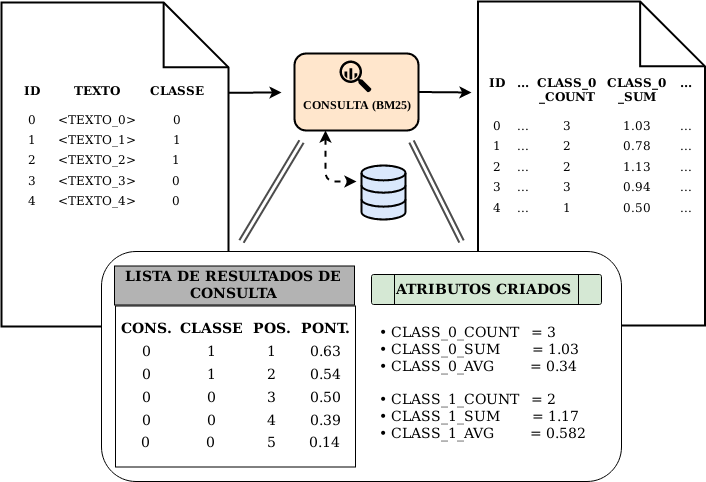
\includegraphics[width=0.9\textwidth]{img/diagrama-consulta-geracao-atributo.png}
    \end{center}
    \vspace{-0.0cm}
    \text{\footnotesize \textbf{Fonte:} O autor.}
    \label{fig:diagrama-cosulta-geração-atributos}
\end{figure}
        \end{columns}
    \end{frame}

    \begin{frame}{\sectiontitle{sec:matmet}}{Atributos de RI sugeridos}
        \begin{table}[H]
    \centering
    \caption{Atributos derivados de RI sugeridos.}
    \begin{tabular}{|p{4.0cm}|l|l|}
        \hline
        \diagbox[width=4.4cm, height=2.0cm]{Agregação}{
            \raisebox{-1.3cm}{
                \rotatebox{90}{
                    \parbox{1.2cm}{\centering Exemplo}
                }
            }
        }  
        & \makecell[l]{Não faz parte da \\ classe da tarefa}
        & \makecell[l]{Faz parte da \\ classe da tarefa}
        \\ \hline
        \makecell[l]{Média aritmética \\ das pontuações}
        & \textbf{CLASS\_0\_BM25\_AVG} 
        & \textbf{CLASS\_1\_BM25\_AVG}  
        \\ \hline
        \makecell[l]{Contagem do número \\ de resultados}
        & \textbf{CLASS\_0\_BM25\_COUNT} 
        & \textbf{CLASS\_1\_BM25\_COUNT}  
        \\ \hline
        \makecell[l]{Soma das \\ pontuações}
        & \textbf{CLASS\_0\_BM25\_SUM} 
        & \textbf{CLASS\_1\_BM25\_SUM}  
        \\ 
        \hline
    \end{tabular}
    \text{\footnotesize \textbf{Fonte:} O autor.}
    \label{tab:lista-atributos-sugeridos}
\end{table}
    \end{frame}

    \begin{frame}{\sectiontitle{sec:matmet}}{Medidas para avaliação de desempenho}
        \vspace{0.2cm}
        \begin{columns}[t]
            \column{0.45\textwidth}
            Medidas de desempenho computacional das ferramentas de armazenamento e indexação:
            \begin{itemize}
                \item \textbf{TIME\_INDEX}: Tempo de execução para indexar o conjunto de treinamento de cada um dos corpus para avaliação elencados;

                \item \textbf{TIME\_QUERY}: Tempo para consulta de cada exemplo do conjunto de teste e geração dos atributos sugeridos para o item específico.
            \end{itemize}

            \column{0.45\textwidth}
            Medidas de desempenho de classificador:
            \begin{itemize}
                \item \textbf{CLF\_ACC}: Acurácia do classificador no conjunto de validação.
                \item \textbf{CLF\_F1}: $F_1$-score do classificador no conjunto de validação.
            \end{itemize}
        \end{columns}
    \end{frame}

    % \subsection{Cronograma}\label{subsec:cronograma}
    % \begin{frame}{\sectiontitle{subsec:cronograma}}{}
    %     \begin{table}[!thb]
	%\huge
    \centering
    \caption{Cronograma das atividades previstas para o TCC II.}
    \begin{adjustbox}{max width=0.75\textwidth}
    \begin{tabular}{p{6.5cm}|c|c|c|c|c|c}
        \toprule
        \textbf{Atividade}
        & Set & Out & Nov & Dez & Jan & Fev
        \\ \hline
        Definição e obtenção dos corpus para avaliação 
        & X   &     &     &     &     &          
        \\ \hline
        Inspeção e seleção das soluções com código fonte disponível
        & X   &     &     &     &     &          
        \\ \hline
        Instalação e familiarização com as ferramentas de arquivamento e indexação
        & X   & X   &     &     &     &          
        \\ \hline
        Indexação do conjunto de treinamento dos corpus
        &     & X   & X   &     &     &          
        \\ \hline
        Adição dos atributos de RI às soluções selecionadas
        &     & X   & X   &     &     &    
        \\ \hline
        Mineração dos dados por meio da reprodução das soluções selecionadas com/sem adição dos atributos de RI
        &     &     & X   & X   & X   &  
        \\ \hline
        Escrita do TCC II                       
        & X   & X   & X   & X   & X   &         
        \\ \hline
        Defesa do TCC II                        
        &     &     &     &     & X   &        
        \\
        \bottomrule
    \end{tabular}
    \end{adjustbox}
    
    \text{\footnotesize \textbf{Fonte:} O autor.}
    \label{tab:cronograma} 
    % \legend{\textbf{Fonte:} O autor.}
\end{table}
    % \end{frame}
\section{Resultados}\label{sec:result}

    \begin{frame}{\sectiontitle{sec:result}}{Configuração experimental}
        \begin{columns}[T]
            \column{0.53\textwidth}
                \centering
                \begin{table}[H]
    \centering
    \caption{Configuração do computador de mesa utilizado neste estudo.}
    % \begin{adjustbox}{max width={\textwidth},keepaspectratio}%
    
    \begin{center}
    \begin{tabular}{|l|p{3.5cm}|}
        \hline
        % \textbf{Posição}  
        % & \makecell[l]{\textbf{Equipe}}
        % & \makecell[l]{\textbf{Repositório de código no site \url{https://github.com/}}}
        % \\ \hline
        Processador
        & Intel(R) Core(TM) i7-4770 CPU @ 3.40GHz
        \\ \hline
        Memória RAM
        & 32370 MB
        \\ \hline
        Sistema Operacional
        & Linux Mint 19.2 Tina
        \\ \hline
        Placa-mãe
        & Gigabyte Z97-D3H
        \\ \hline
        Gráficos
        & Mesa DRI Intel(R) Haswell Desktop
        \\ \hline
        Disco
        & HP SSD EX920 512GB
        \\ \hline
    \end{tabular}
    \end{center}
    % \end{adjustbox}
    \text{\footnotesize \textbf{Fonte:} O autor.}
    \label{tab:sistema-computacional}
\end{table}

                \raggedright
                Todo código fonte utilizado está disponível em: \hyperlink{https://github.com/ruanmed/tcc-ii-ir-features-text-mining/}{https://github.com/ruanmed/tcc-ii-ir-features-text-mining/}.
            \column{0.45\textwidth}
                \begin{itemize}
                    \item Geração dos atributos de RI utilizando as ferramentas com os seguintes parâmetros:
                    \begin{itemize}
                        \vspace{-0.5cm}
                        \item $k_1 = 1.2$;
                        \item $k_3 = 0$
                        \item $b = 0.75$; e
                        \item $\text{top-}k = 100$.
                    \end{itemize}
                    \item Os scripts para o estudo foram feitos na linguagem de programação Python 3.7.5 com o ambiente VSCodium.

                    \item RNG\footnote{gerador de números aleatórios} fixo para permitir reprodutibilidade.

                    \item As dependências soluções selecionadas foram instaladas: bibliotecas adicionais do Python e download de arquivos específicos para essas bibliotecas.
                \end{itemize}
        \end{columns}
    \end{frame}

    \begin{frame}{\sectiontitle{sec:result}}{Visão geral das soluções}
            Foram selecionadas as seguintes soluções para reprodução e posterior adição dos atributos de RI:
            \begin{itemize}
                \item DB\_HYPERPARTISAN:
                    \begin{itemize}
                        \item 1\_bertha
                        \item 4\_tom
                    \end{itemize}
                \item DB\_AUTHORPROF:
                    \begin{itemize}
                        \item 2\_daneshvar18
                    \end{itemize}
            \end{itemize}
    \end{frame}

    \begin{frame}{\sectiontitle{sec:result}}{Visão geral das soluções: 1\_bertha}
        Solução do corpus DB\_HYPERPARTISAN.
        
        \begin{figure}[h]
    \centering
    \caption{Arquitetura de sistema da solução 1\_bertha após adaptação.}
    \begin{center}
        \begin{overprint}
            \onslide<1>\centering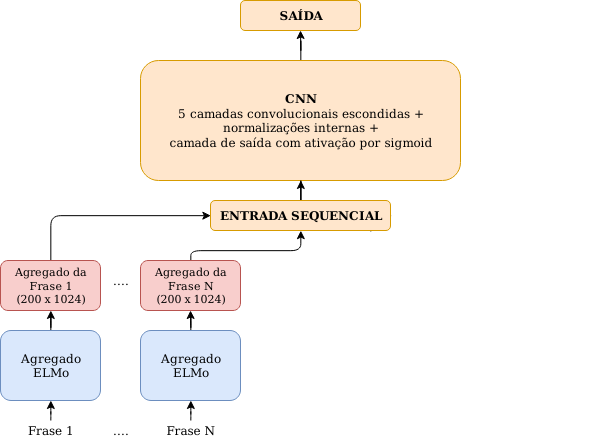
\includegraphics[width=0.50\textwidth]{img/1-bertha-arquitetura-sem-ri.png}\onslide<2>\centering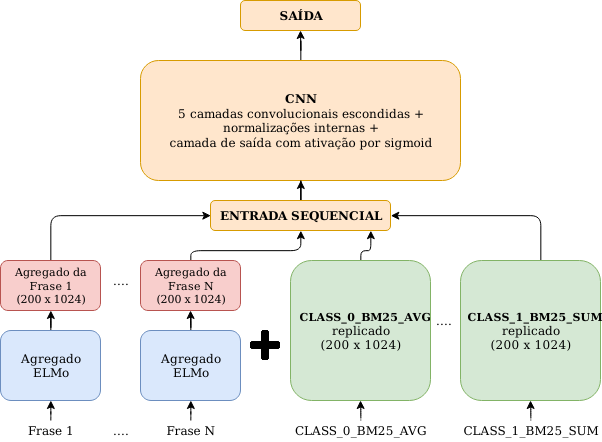
\includegraphics[width=0.50\textwidth]{img/1-bertha-arquitetura-com-ri.png}
        \end{overprint}
    \end{center}
    \vspace{-0.0cm}
    \text{\footnotesize \textbf{Fonte:} O autor.}
    \label{fig:1-bertha-arquitetura-com-ri}
\end{figure}

    \end{frame}

    \begin{frame}{\sectiontitle{sec:result}}{Visão geral das soluções: 4\_tom}
        Solução do corpus DB\_HYPERPARTISAN.
        
        \begin{figure}[h]
    \centering
    \caption{Arquitetura de sistema da solução 4\_tom após adaptação.}
    \begin{center}
        \begin{overprint}
            \onslide<1>\centering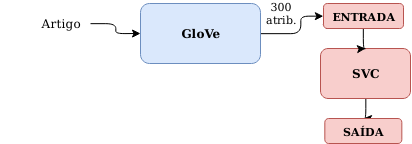
\includegraphics[width=0.68\textwidth]{img/4-tom-arquitetura-sem-ri.png}\onslide<2>\centering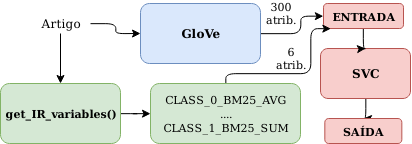
\includegraphics[width=0.68\textwidth]{img/4-tom-arquitetura-com-ri.png}
        \end{overprint}
    \end{center}
    \vspace{-0.0cm}
    \text{\footnotesize \textbf{Fonte:} O autor.}
    \label{fig:4-tom-arquitetura-com-ri}
\end{figure}
        
    \end{frame}

    \begin{frame}{\sectiontitle{sec:result}}{Visão geral das soluções: 2\_daneshvar18}
        Solução do corpus DB\_AUTHORPROF.
        
        \begin{figure}[h]
    \centering
    \caption{Arquitetura de sistema da solução 2\_daneshvar18 após adaptação.}
    \begin{center}
        \begin{overprint}
            \onslide<1>\centering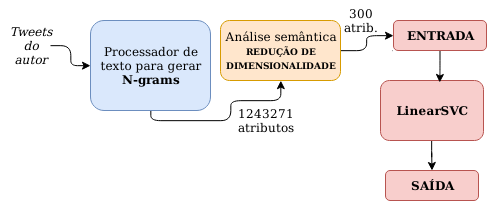
\includegraphics[width=0.75\textwidth]{img/2-daneshvar18-arquitetura-sem-ri.png}\onslide<2>\centering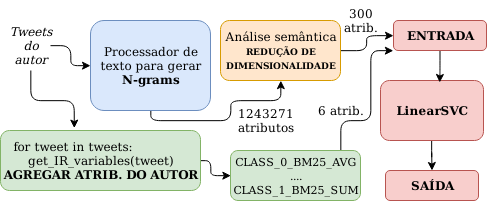
\includegraphics[width=0.75\textwidth]{img/2-daneshvar18-arquitetura-com-ri.png}
        \end{overprint}
    \end{center}
    \vspace{-0.0cm}
    \text{\footnotesize \textbf{Fonte:} O autor.}
    \label{fig:2-daneshvar18-arquitetura-com-ri}
\end{figure}
        
    \end{frame}

    \begin{frame}{\sectiontitle{sec:result}}{Visão geral das soluções: resumo}
        As principais características das soluções selecionadas estão na Tabela \ref{tab:resumo-soluções}.
        
        \begin{table}[!thb]
	%\huge
    \centering
    \caption{Resumo dos detalhes das soluções selecionadas.}
    \begin{adjustbox}{max width={\textwidth},keepaspectratio}%
    \begin{tabular}{|l|c|c|c|c|c|}
        % \toprule
        \hline
        \textbf{Solução}
        & \textbf{Pré-processamento} & \textbf{Núm. atrib.} & \textbf{Redução dim.} 
        & \textbf{Núm. atrib. após}  & \textbf{Classificador}
        \\ \hline
        1\_bertha        
        & ELMo          & 200 x 1024        & Não
        & 200 x 1024    & CNN (5 cam. esc.) 
        \\ \hline
        4\_tom
        & GloVe         & 300               & Não
        & 300           & SVC                
        \\ \hline
        2\_daneshvar18
        & N-gram palavras+caracteres & 1243271           & Sim
        & 300           & LinearSVC          
        \\ 
        \hline
        % \bottomrule
    \end{tabular}
    \end{adjustbox}
    \text{\footnotesize \textbf{Fonte:} O autor.}
    \label{tab:resumo-soluções} 
    % \legend{\textbf{Fonte:} O autor.}
\end{table}


    \end{frame}

    \begin{frame}{\sectiontitle{sec:result}}{Desempenho das ferramentas de armazenamento e indexação}
        \begin{columns}
            \column{0.30\textwidth} 
            O cálculo das medidas TIME\_INDEX e TIME\_QUERY foi auxiliado com a implementação de uma classe chamada \textit{IndexToolManager} que abstrai a indexação e o cálculo das variáveis de RI com as ferramentas.
            
            A utilização dela concentrou as funções para acesso e manipulação, quando disponíveis, aos dados das ferramentas de armazenamento e indexação, centralização das diferentes bibliotecas do Python já disponíveis para interagircom o ArangoDB e com o Elasticsearch, python-arango e elasticsearch-py respectivamente.
            Esta classe foi central para todo o estudo, inclusive para geração dos atributos de RI.

            \column{0.65\textwidth}
                \vspace{-1.0cm}
                \inputminted[bgcolor=bg, fontsize=\scriptsize,
                baselinestretch=1, tabsize=2, breaklines]{python}{codes/indextoolmanager-reduced.py}
        \end{columns}
    \end{frame}
    
    \begin{frame}{\sectiontitle{sec:result}}{Tempo de indexação}
        \begin{columns}
            \column{0.30\textwidth} 
            O cálculo da medida TIME\_INDEX foi feito com o script \texttt{time\_index.py}, o qual utilizou da classe \textit{IndexToolManager} em duas funções feitas para executar a indexação dos corpus DB\_AUTHORPROF e DB\_HYPERPARTISAN nas 3 ferramentas, ArangoDB, Elasticsearch e Zettair.
            
            A função principal do script \texttt{time\_index.py} possui nome \textit{measure\_TIME\_INDEX}, e um trecho dela pode ser visto ao lado.

            \column{0.65\textwidth}
                \vspace{-1.0cm}
                \inputminted[bgcolor=bg, fontsize=\scriptsize,
                baselinestretch=1, tabsize=2, breaklines]{python}{codes/function-measure-TIME-INDEX.py}
        \end{columns}
    \end{frame}
    
    \begin{frame}{\sectiontitle{sec:result}}{Tempo de indexação}
        \begin{columns}[T]
            \column{0.50\textwidth}
                \vspace{-0.5cm}
                \begin{figure}[h]
    \centering
    \caption{Medidas de desempenho TIME\_INDEX mensuradas para as ferramentas de armazenamento e indexação, com inserções feitas em lote.}
    \vspace{-0.0cm}
    \begin{center}
        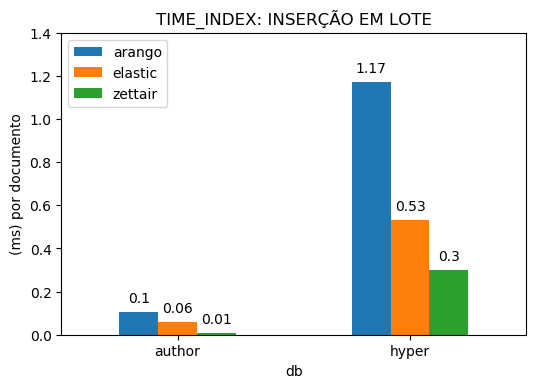
\includegraphics[width=1.0\textwidth]{img/time-index-bulk.png}
    \end{center}
    \vspace{-0.0cm}
    \text{\footnotesize \textbf{Fonte:} O autor.}
    \label{fig:time-index-bulk}
\end{figure}
            \column{0.50\textwidth}
                \vspace{-0.5cm}
                \begin{figure}[h]
    \centering
    \caption{Medidas de desempenho TIME\_INDEX mensuradas para as ferramentas de armazenamento e indexação, com inserções unitárias.}
    \vspace{-0.0cm}
    \begin{center}
        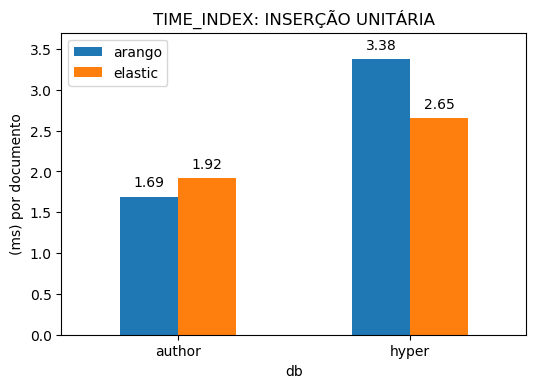
\includegraphics[width=1.0\textwidth]{img/time-index-individual.png}
    \end{center}
    \vspace{-0.0cm}
    \text{\footnotesize \textbf{Fonte:} O autor.}
    \label{fig:time-index-individual}
\end{figure}
        \end{columns}
    \end{frame}
    
    \begin{frame}{\sectiontitle{sec:result}}{Tempo de consulta}
        \begin{columns}
            \column{0.30\textwidth} 
            Para medir o TIME\_QUERY utilizando cada ferramenta durante a execução das soluções foi necessário adaptar os códigos das soluções para fazer o registro do tempo que cada consulta, e posterior geração dos atributos de RI, levou.

			A utilização dos métodos implementados na classe \textit{IndexToolManager} podem ser vistos no trecho disposto a seguir do script Python \texttt{feat\_GloVe.ipynb} da solução 4\_tom adaptada.

            \column{0.70\textwidth}
                \vspace{-1.0cm}
                \inputminted[bgcolor=bg, fontsize=\scriptsize,
                baselinestretch=1, tabsize=1,obeytabs,showtabs, breaklines]{python}{codes/time-query-calculation-4-tom.py}
        \end{columns}
    \end{frame}

    \begin{frame}{\sectiontitle{sec:result}}{Tempo de consulta}
        \vspace{-0.5cm}
        \begin{figure}[h]
    \centering
    \caption{Medidas de desempenho TIME\_QUERY mensuradas para consulta e criação dos 6 atributos de RI sugeridos, utilizando as ferramentas de armazenamento e indexação.}
    \vspace{-0.0cm}
    \begin{center}
        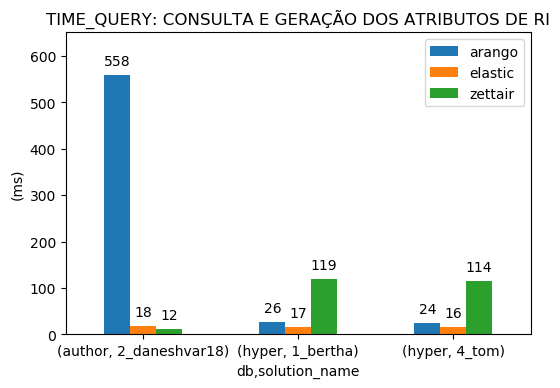
\includegraphics[width=0.60\textwidth]{img/time-query.png}
    \end{center}
    \vspace{-0.0cm}
    \text{\footnotesize \textbf{Fonte:} O autor.}
    \label{fig:time-query}
\end{figure}
    \end{frame}

    \begin{frame}{\sectiontitle{sec:result}}{Desempenho dos classificadores com atributos de RI}
        O desempenho dos classificadores foi mensurado conforme as medidas CLF\_ACC e CLF\_F1 estabelecidas.

        As soluções originais foram reproduzidas, comparadas com os resultados divulgados nas páginas das competições, e então as soluções foram reproduzidas com as adaptações para incluiros atributos de RI gerados por cada uma das ferramentas.
    \end{frame}

    \begin{frame}{\sectiontitle{sec:result}}{DB\_HYPERPARTISAN: reprodução das soluções originais}
        O conjunto de validação da competição não foi disponibilizado ao público.
        Foi realizado o \textit{holdout} no conjunto de treinamento, 430 artigos foram separados para o conjunto de treinamento e 215 para validação.

        As medidas das soluções reproduzidas se encontram na Tabela \ref{tab:reprodução-db-hyperpartisan}.
        
        \begin{table}[!thb]
	%\huge
    \centering
    \caption{Comparação das medidas das soluções do corpus DB\_HYPERPARTISAN divulgadas pelas competição e das reproduções.}
    \begin{adjustbox}{max width={\textwidth},keepaspectratio}%
    \begin{tabular}{|l|c|c|c|c|c|}
        % \toprule
        \hline
        \multirow{2}{*}{\textbf{Solução}}
        & \multicolumn{2}{|c|}{\textbf{Acurácia}}
        & \multicolumn{2}{|c|}{\textbf{$F_1$-Score}}
        \\ \cline{2-5}    
        & Competição    & Reprodução
        & Competição    & Reprodução 
        \\ \hline
        1\_bertha        
        & 0,822         & 0,814
        & 0,809         & 0,762
        \\ \hline
        4\_tom
        & 0,806         & 0,809
        & 0,790         & 0,707              
        \\ 
        \hline
        % \bottomrule
    \end{tabular}
    \end{adjustbox}
    \text{\footnotesize \textbf{Fonte:} O autor.}
    \label{tab:reprodução-db-hyperpartisan} 
    % \legend{\textbf{Fonte:} O autor.}
\end{table}


        Relação de superioridade das soluções na competição se manteve nas reproduções.

    \end{frame}

    
    \begin{frame}{\sectiontitle{sec:result}}{DB\_HYPERPARTISAN: desempenho das soluções com atributos de RI}
        \begin{columns}[T]
            \column{0.50\textwidth}
                \vspace{-0.5cm}
                \begin{figure}[h]
    \centering
    \caption{Desempenho CLF\_ACC das soluções do corpus DB\_HYPERPARTISAN.}
    \vspace{-0.0cm}
    \begin{center}
        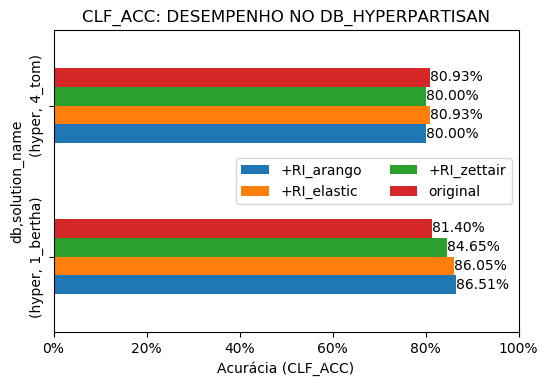
\includegraphics[width=1.0\textwidth]{img/clf-acc-bars-hyperpartisan.png}
    \end{center}
    \vspace{-0.0cm}
    \text{\footnotesize \textbf{Fonte:} O autor.}
    \label{fig:clf-acc-bars-hyperpartisan}
\end{figure}
            \column{0.50\textwidth}
                \vspace{-0.5cm}
                \begin{figure}[h]
    \centering
    \caption{Desempenho CLF\_F1 das soluções do corpus DB\_HYPERPARTISAN.}
    \vspace{-0.0cm}
    \begin{center}
        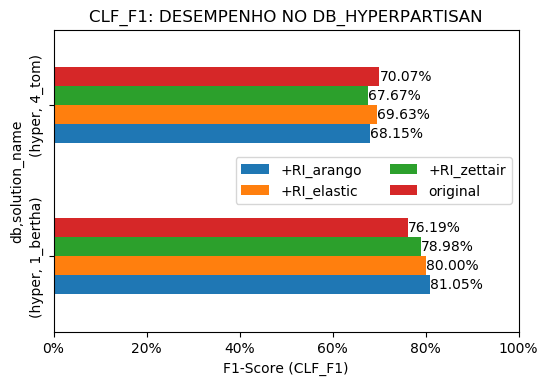
\includegraphics[scale=0.75]{img/clf-f1-bars-hyperpartisan.png}
    \end{center}
    \vspace{-0.0cm}
    \text{\footnotesize \textbf{Fonte:} O autor.}
    \label{fig:clf-f1-bars-hyperpartisan}
\end{figure}
        \end{columns}
    \end{frame}
    
    \begin{frame}{\sectiontitle{sec:result}}{DB\_HYPERPARTISAN: reprodução da solução 4\_tom com diferentes C}
        \begin{columns}[T]
            \column{0.50\textwidth}
                \vspace{-0.5cm}
                \begin{figure}[h]
    \centering
    \caption{Desempenho CLF\_ACC da solução 4\_tom para diferentes valores de refinamento da função custo, parâmetro C do classificador SVC.}
    \vspace{-0.0cm}
    \begin{center}
        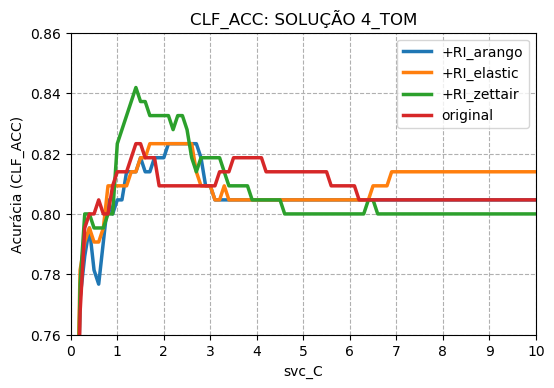
\includegraphics[width=1.0\textwidth]{img/clf-acc-4-tom.png}
    \end{center}
    \vspace{-0.0cm}
    \text{\footnotesize \textbf{Fonte:} O autor.}
    \label{fig:clf-acc-4-tom}
\end{figure}
            \column{0.50\textwidth}
                \vspace{-0.5cm}
                \begin{figure}[h]
    \centering
    \caption{Desempenho CLF\_F1 da solução 4\_tom para diferentes valores de refinamento da função custo, parâmetro C do classificador SVC.}
    \vspace{-0.0cm}
    \begin{center}
        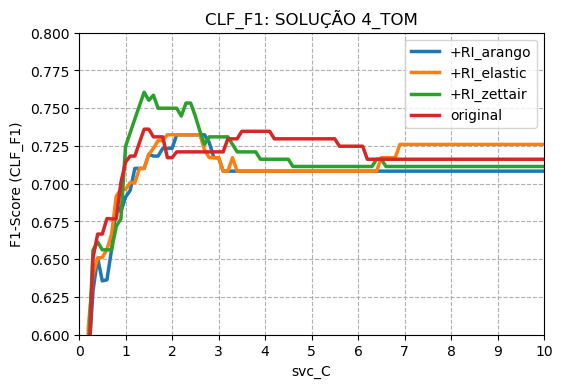
\includegraphics[width=1.0\textwidth]{img/clf-f1-4-tom.png}
    \end{center}
    \vspace{-0.0cm}
    \text{\footnotesize \textbf{Fonte:} O autor.}
    \label{fig:clf-f1-4-tom}
\end{figure}
        \end{columns}
    \end{frame}

    \begin{frame}{\sectiontitle{sec:result}}{DB\_HYPERPARTISAN: reprodução da solução 4\_tom com diferentes C}
        % Uma rápida análise dos gráficos permite perceber que os melhores valores do parâmetro C agora se encontram na faixa de 1,0 a 3,0 para as reproduções, tanto em termos de CLF\_ACC quanto de CLF\_F1.
        % O valor de $C = 0,9$ de fato não está entre os melhores possíveis para o classificador.
        
        Nota-se que, mesmo com a adição dos atributos de RI, utilizando tanto o ArangoDB quanto o Elasticsearch, o classificador em nenhum momento consegue superar o melhor valor de C do classificador original, porém, com adição dos atributos de RI gerados pelo Zettair é atingido o melhor valor.

        Os valores máximos atingidos com os respectivos valores de C estão dispostos na Tabela \ref{tab:reprodução-4-tom-c}.
        
        \begin{table}[!thb]
	%\huge
    \centering
    \caption{Melhores valores de CLF\_ACC e CLF\_F1 do classificador SVC da solução 4\_tom após reproduzida com diferentes valores de C.}
    \begin{adjustbox}{max width={\textwidth},keepaspectratio}%
    \begin{tabular}{|l|c|c|c|}
        % \toprule
        \hline
        \textbf{Solução}
        & \textbf{C}
        & \textbf{Acurácia}
        & \textbf{$F_1$-Score}
        \\ \hline
        original        
        & 1,4   & 0,8233   & 0,7361 
        \\ \hline
        +RI\_arango
        & 2,1   & 0,8233    & 0,7324          
        \\ \hline
        +RI\_elastic
        & 1,9   & 0,8233    & 0,7324        
        \\ \hline
        +RI\_zettair
        & 1,4   & \textbf{0,8419}    & \textbf{0,7606}          
        \\ 
        \hline
        % \bottomrule
    \end{tabular}
    \end{adjustbox}
    \text{\footnotesize \textbf{Fonte:} O autor.}
    \label{tab:reprodução-4-tom-c} 
    % \legend{\textbf{Fonte:} O autor.}
\end{table}

    \end{frame}

    \begin{frame}{\sectiontitle{sec:result}}{DB\_AUTHORPROF: reprodução da solução original}
        A solução 2\_daneshvar18 foi reproduzida sem nenhuma adaptação para comparação com os valores que se encontram na página da competição.
        
        Na Tabela \ref{tab:reprodução-db-authorprof} está a medida de acurácia divulgada na página da competição \cite{PAN_APCLEF_2018} junto com as medidas da reprodução feitas do mesmo modo que a submissão original, treinamento com os tweets de 3000 autores de língua inglesa e validação com os tweets de 1900 autores de língua inglesa.
        
        \begin{table}[!thb]
	%\huge
    \centering
    \caption{Comparação das medidas da solução 2\_daneshvar18 do corpus DB\_AUTHORPROF divulgadas pela competição e da reprodução da solução.}
    \begin{adjustbox}{max width={\textwidth},keepaspectratio}%
    \begin{tabular}{|l|c|c|c|c|c|}
        % \toprule
        \hline
        \multirow{2}{*}{\textbf{Solução}}
        & \multicolumn{2}{|c|}{\textbf{Acurácia}}
        & \multicolumn{2}{|c|}{\textbf{$F_1$-Score}}
        \\ \cline{2-5}    
        & Competição    & Reprodução
        & Competição    & Reprodução 
        \\ \hline
        2\_daneshvar18        
        & 0,8221        & 0,822105	
        & --            & 0,820785
        \\ 
        \hline
        % \bottomrule
    \end{tabular}
    \end{adjustbox}
    \text{\footnotesize \textbf{Fonte:} O autor.}
    \label{tab:reprodução-db-authorprof} 
    % \legend{\textbf{Fonte:} O autor.}
\end{table}


        O resultado de acurácia da solução reproduzida truncado em 4 dígitos é o mesmo valor divulgado na página da competição.s
    \end{frame}

    \begin{frame}{\sectiontitle{sec:result}}{DB\_AUTHORPROF: desempenho da solução com atributos de RI}
        \vspace{-0.5cm}
        \begin{figure}[h]
    \centering
    \caption{Desempenho CLF\_F1 e CLF\_ACC da solução reproduzida para o corpus DB\_AUTHORPROF.}
    \vspace{-0.0cm}
    \begin{center}
        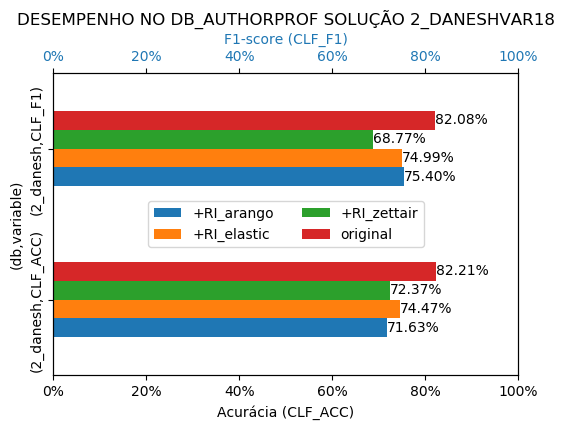
\includegraphics[width=0.6\textwidth]{img/clf-bars-authorprof.png}
    \end{center}
    \vspace{-0.0cm}
    \text{\footnotesize \textbf{Fonte:} O autor.}
    \label{fig:clf-bars-authorprof}
\end{figure}
    \end{frame}

    \begin{frame}{\sectiontitle{sec:result}}{DB\_AUTHORPROF: reprodução da solução 2\_daneshvar18 com diferentes C}
        \begin{columns}[T]
            \column{0.50\textwidth}
                \vspace{-0.5cm}
                \begin{figure}[h]
    \centering
    \caption{Desempenho CLF\_ACC da solução 2\_daneshvar18 para diferentes valores de refinamento da função custo, parâmetro C do classificador LinearSVC.}
    \vspace{-0.0cm}
    \begin{center}
        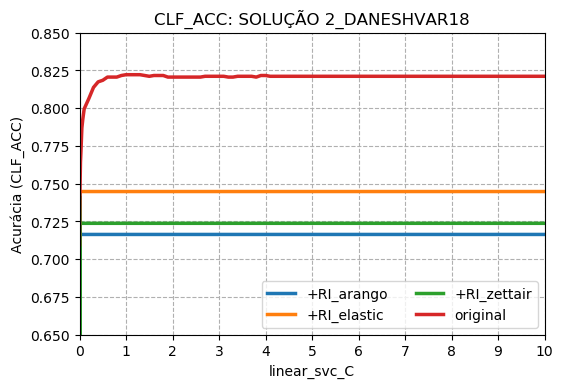
\includegraphics[scale=0.75]{img/clf-acc-2-daneshvar18.png}
    \end{center}
    \vspace{-0.0cm}
    \text{\footnotesize \textbf{Fonte:} O autor.}
    \label{fig:clf-acc-2-daneshvar18}
\end{figure}
            \column{0.50\textwidth}
                \vspace{-0.5cm}
                \begin{figure}[h]
    \centering
    \caption{Desempenho CLF\_F1 da solução 2\_daneshvar18 para diferentes valores de refinamento da função custo, parâmetro C do classificador LinearSVC.}
    \vspace{-0.0cm}
    \begin{center}
        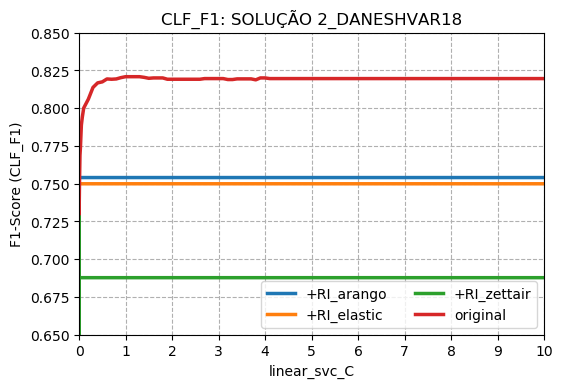
\includegraphics[width=1.0\textwidth]{img/clf-f1-2-daneshvar18.png}
    \end{center}
    \vspace{-0.0cm}
    \text{\footnotesize \textbf{Fonte:} O autor.}
    \label{fig:clf-f1-2-daneshvar18}
\end{figure}
        \end{columns}
    \end{frame}

    \begin{frame}{\sectiontitle{sec:result}}{DB\_AUTHORPROF: reprodução da solução 2\_daneshvar18 com atributos de RI escalonados}
        \begin{columns}[T]
            \column{0.50\textwidth}
                \vspace{-0.5cm}
                \begin{figure}[h]
    \centering
    \caption{Desempenho CLF\_ACC da solução 2\_daneshvar18 para diferentes valores de refinamento da função custo, parâmetro C do classificador LinearSVC com atributos de RI escalonados pelo MinMaxScaler.}
    \vspace{-0.0cm}
    \begin{center}
        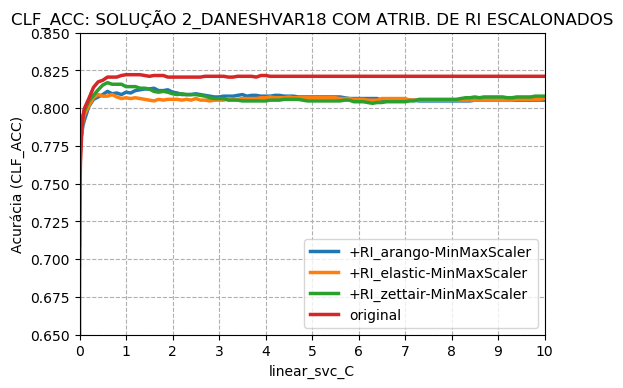
\includegraphics[width=1.0\textwidth]{img/clf-acc-2-daneshvar18-ir-scaled.png}
    \end{center}
    \vspace{-0.0cm}
    \text{\footnotesize \textbf{Fonte:} O autor.}
    \label{fig:clf-acc-2-daneshvar18-ir-scaled}
\end{figure}
            \column{0.50\textwidth}
                \vspace{-0.5cm}
                \begin{figure}[h]
    \centering
    \caption{Desempenho CLF\_F1 da solução 2\_daneshvar18 para diferentes valores de refinamento da função custo, parâmetro C do classificador LinearSVC com atributos de RI escalonados pelo MinMaxScaler.}
    \vspace{-0.0cm}
    \begin{center}
        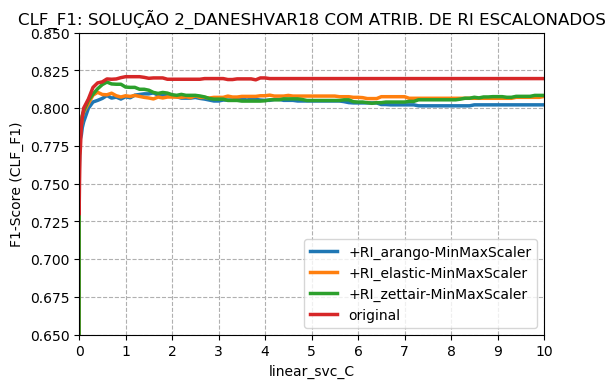
\includegraphics[scale=0.75]{img/clf-f1-2-daneshvar18-ir-scaled.png}
    \end{center}
    \vspace{-0.0cm}
    \text{\footnotesize \textbf{Fonte:} O autor.}
    \label{fig:clf-f1-2-daneshvar18-ir-scaled}
\end{figure}
        \end{columns}
    \end{frame}

    \begin{frame}{\sectiontitle{sec:result}}{DB\_AUTHORPROF: reprodução da solução 2\_daneshvar18 com atributos de RI escalonados}
        % Uma rápida análise dos gráficos permite perceber que os melhores valores do parâmetro C agora se encontram na faixa de 1,0 a 3,0 para as reproduções, tanto em termos de CLF\_ACC quanto de CLF\_F1.
        % O valor de $C = 0,9$ de fato não está entre os melhores possíveis para o classificador.
        
        Ainda assim o desempenho continuou abaixo da reprodução da solução original.

        Na Tabela \ref{tab:reprodução-2-daneshvar18-c} podem ser vistos os valores máximos atingidos com os respectivos valores de C.
        
        \begin{table}[!thb]
	%\huge
    \centering
    \caption{Melhores valores de CLF\_ACC e CLF\_F1 do classificador LinearSVC da solução 2\_daneshvar18 após reproduzida com diferentes valores de C, com atributos de RI escalonados pelo MinMaxScaler.}
    \begin{adjustbox}{max width={\textwidth},keepaspectratio}%
    \begin{tabular}{|l|c|c|c|}
        % \toprule
        \hline
        \textbf{Solução}
        & \textbf{C}
        & \textbf{Acurácia}
        & \textbf{$F_1$-Score}
        \\ \hline
        original        
        & 1,0   & \textbf{0,822105}   & \textbf{0,820785}
        \\ \hline
        +RI\_arango
        & 1,6   & 0,813158   & 0,810059          
        \\ \hline
        +RI\_elastic
        & 0,4   & 0,808947    & 0,810444
        \\ \hline
        +RI\_zettair
        & 0,6   & 0,816842	    & 0,817227
        \\ 
        \hline
        % \bottomrule
    \end{tabular}
    \end{adjustbox}
    \\
    \text{\footnotesize \textbf{Fonte:} O autor.}
    \label{tab:reprodução-2-daneshvar18-c} 
    % \legend{\textbf{Fonte:} O autor.}
\end{table}


        O melhor desempenho com os atributos de RI é quando gerado pelo Zettair, no entanto ainda assim fica abaixo da solução original.
    \end{frame}

\section{Considerações finais e trabalhos futuros}\label{sec:consfinais}
    \begin{frame}{\sectiontitle{sec:consfinais}}{}
        \begin{columns}[t]
            \column{0.50\textwidth}
            \vspace{-0.5cm}
            % \setlength{\itemindent}{0.1em}
            \begin{itemize}
                \setlength{\leftmargin}{-1.5cm}
                \item  Avaliação do desempenho de atributos oriundos da área de Recuperação de Informação em tarefas de Mineração de Texto, com enfoque em atributos gerados pela função BM25;

                \item Zettair foi a ferramenta testada mais rápida, porém com limitações;

                \item Elasticsearch foi mais rápido no geral;
                
                \item ArangoDB apresenta lentidão para calcular BM25 para corpus grandes;
                
                \item Comprovação das medidas do ranking final da competição do corpus DB\_AUTHORPROF para a solução 2\_daneshvar18;
                
                \item Falta do conjunto de validação final da competição impossibilitou comprovar as medidas do ranking final do corpus DB\_HYPERPARTISAN;
            \end{itemize}

            \column{0.53\textwidth}
            \vspace{-0.5cm}
            \begin{itemize}
                
                \item Desempenho de classificador com atributos de RI:
                    \begin{itemize}
                        \item Solução 1\_bertha do DB\_HYPERPARTISAN apresentou ganho de desempenho ao adicionar os atributos, das 3 ferramentas;
                        \item Não houve ganho inicial de desempenho com a solução 4\_tom utilizando os atributos de RI;
                        \item Adicionar os atributos gerados pelo Zettair produz um ganho de desempenho quando o melhor valor do parâmetro C, do SVC da solução 4\_tom, é selecionado;
                        \item O classificador LinearSVC da solução 2\_daneshvar18 não obteve nenhum ganho de desempenho, nem mesmo ao ser feita a análise e seleção do parâmetro C do classificador;
                        \item Mesmo com o reparo de magnitude por meio do escalonador MinMaxScaler, e nova análise e seleção do parâmetro C do classificador, não foi obtido ganho de desempenho na solução 2\_daneshvar18.
                    \end{itemize}
                
            \end{itemize}
        \end{columns}
    \end{frame}

    \begin{frame}{\sectiontitle{sec:consfinais}}{Desempenho dos atributos de RI}
        \begin{itemize}
            \item Os 6 atributos de RI sugeridos nesse estudo proporcionaram \textbf{ganho de desempenho somente} para classificações do corpus DB\_HYPERPARTISAN, um \textbf{corpus pequeno com documentos extensos}.
            Os atributos de RI funcionaram melhor com o classificador CNN, e para o classificador SVC somente o Zettair proporcionou ganho de desempenho;
            
            \item No corpus DB\_AUTHORPROF, um \textbf{corpus grande com documentos curtos}, com o classificador LinearSVC, \textbf{os atributos de RI causaram perda de desempenho};
            
            \item São necessários mais estudos para corroborar os resultados obtidos, com outros corpus e classificadores.

        \end{itemize}
    \end{frame}
    \begin{frame}{\sectiontitle{sec:consfinais}}{Trabalhos futuros}
        \begin{itemize}
            \item Reproduzir a solução 2\_daneshvar18 com outras variações nos parâmetros do classificador LinearSVC;
            
            \item Reproduzir mais uma das soluções do corpus DB\_AUTHORPROF disponíveis online;
            
            \item Analise de diferentes valores que influenciem somente nos atributos de RI gerados, o top-$k$ e os parâmetros $k_1$, $k_3$ e $b$ reproduzindo-os para os mesmos corpus.

            \item Separação dos corpus em 3 pedaços para trabalhar com um índice isolado para geração dos atributos de RI.
            O primeiro pedaço seria utilizado para para treinamento do classificador, o segundo pedaço seria utilizado como o índice para geração dos atributos derivados da função BM25 para o primeiro pedaço, e o terceiro pedaço ficaria para teste/validação do classificador.
        \end{itemize}
    \end{frame}

\mode<presentation>{%% Modo apresentação --- Referências
  \section{Referências}\label{sec:ref}%
  \begin{frame}[allowframebreaks]{\sectiontitle{sec:ref}}{~}%
    \printbibliography[heading = none]%
  \end{frame}%
}

\mode<article>{\printbibliography}%% Modo artigo --- Referências

\section*{Agradecimentos}\label{sec:agrad}

    % \begin{frame}[c]{\sectiontitle{sec:agrad}}{\mode<presentation>{~}}
    %     Pelo apoio recebido para o desenvolvimento deste trabalho e a participação neste evento:
    %     \mode<presentation>{\vfill}%% Modo apresentação --- Espaçamento vertical
    %     \begin{center}
    %     
\includegraphics[height = \logoheight]{./Logos/logo-capes}
    %     \hfill
    %     
\includegraphics[height = \logoheight]{./Logos/logo-cnpq}
    %     \hfill
    %     
\includegraphics[height = \logoheight]{./Logos/logo-fa}
    %     \mode<presentation>{\vfill}%% Modo apresentação --- Espaçamento vertical
    %     
\includegraphics[height = \logoheight]{./Logos/logo-utfpr}
    %     \end{center}
    % \end{frame}

    \mode<presentation>{%% Modo apresentação --- Agradecimentos
    \begin{frame}[c]{\sectiontitle{sec:agrad}}{~}%
        \vfill%
        \begin{center}%
          \begin{Huge}%
            Por sua atenção!%
          \end{Huge}%
        \end{center}%
        \vfill%
        % \begin{block}{Declaração de Responsabilidade}%
        %   O(s) autor(es) é(são) o(s) único(s) responsável(eis) pelo material impresso contido neste documento.%
        % \end{block}%
    \end{frame}%
    }

\mode<article>{%% Modo artigo --- Declaração de responsabilidade
    \section*{Declaração de Responsabilidade}%
    O(s) autor(es) é(são) o(s) único(s) responsável(eis) pelo material impresso contido neste documento.%
}

%% Fim do documento
\end{document}
